\documentclass[11pt]{article}
\usepackage[utf8]{inputenc}
\usepackage[T1]{fontenc}
\usepackage{lmodern}
\usepackage[a4paper,margin=1in]{geometry}
\usepackage{amsmath,amssymb}
\usepackage{booktabs,tabularx,array,multirow}
\usepackage{graphicx}
\usepackage[numbers,sort&compress]{natbib}
\usepackage{xcolor}
\usepackage[colorlinks=true,linkcolor=blue!50!black,citecolor=blue!50!black,urlcolor=blue!50!black]{hyperref}
\usepackage{xurl}
\usepackage{microtype}
\usepackage{caption}
\usepackage{float}
\captionsetup{font=small,labelfont=bf}
\newcommand{\Hzero}{H_{0}}
\newcommand{\Hone}{H_{1}}
\newcolumntype{L}[1]{>{\raggedright\arraybackslash}p{#1}}
\newcolumntype{R}{>{\raggedleft\arraybackslash}X}
\emergencystretch=2em

\title{\textbf{No Universal AI Dominance}\\[4pt]
\large A Multi-Dimensional Falsification Test of Vendor, Paradigm and Origin Dominance\\ in Global LLM Adoption}
\author{Rodrigo F. A. P. Oliveira\\ \small CESAR School, Recife, Brazil\\ \small \texttt{rfapo@cesar.school}}
\date{November 2026}

\begin{document}
\maketitle

\begin{abstract}
\noindent Public debate treats large language models (LLMs) as a market with a dominant vendor, paradigm (closed or open weights) or country of origin. We state dominance as the null hypothesis, $\Hzero$: \emph{one entity holds at least half of the market in every adoption dimension}, and test it on 61 data sources and 53 scholarly works covering consumer attention, users, revenue, developer volume and enterprise spend. On single-source data $\Hzero$ is rejected: no vendor reaches 50\% in more than one of five dimensions, and a pooled test calibrated at the least favourable point of $\Hzero$ gives $p$ between 0.0002 and 0.018. At the paradigm and origin levels the test rejects dominance by open weights and by Chinese labs, but not by closed weights or by US labs. The vendor-level rejection is fragile in three ways, which we report with equal weight. With the source most favourable to $\Hzero$ in each dimension, $p$ rises to 0.07--0.16. If, on that reading, Google and Anthropic are counted as one bloc because of Google's 13.7\% stake, a 30\% threshold is met in all five dimensions. Upstream, one firm holds 75--86\% of AI accelerators. Within candidate relevant markets concentration is high (HHI above 1{,}800 in six of nine metrics). Local dominance is not rejected for consumer assistants outside China (OpenAI: 46--79\% in four readings, above 50\% in all 13 months of a panel while losing 19 points) or for enterprise model spend (a leader near or above 50\% in five sources, which disagree on whether it is Anthropic or OpenAI); for Chinese consumer apps it depends on the tracker. Developer inference has no stable leader: three in 13 months. Open-weight families repeat the pattern, and because anyone can serve released weights, Chinese families supply 90\% of open-weight gateway tokens while US-headquartered sellers serve about 58\%. A claim of dominance should name its unit, its market and its source. Data are secondary; code is provided.
\end{abstract}

\noindent\textbf{Keywords:} large language models; market concentration; technology diffusion; open-weight models; Herfindahl--Hirschman index; AI adoption; Global South.

\section{Introduction}

Three claims of dominance circulate about LLMs. The first is about vendors: one company, usually OpenAI, ``owns'' the market. The second is about paradigms: either closed frontier models have won, or cheap open-weight models have. The third is about origin: either US or Chinese labs dominate global use. Each claim is usually supported by a single metric. Web-traffic studies find that ChatGPT took 77\% of visits to the top 60 generative AI tools in April 2025 \cite{liu2025who} and that US models captured about 93\% of global LLM site visits in August 2025 \cite{wang2026uschina}. Gateway telemetry finds the opposite ranking for 2026, with open-weight models from Chinese labs processing most tokens \cite{openrouter2026tokens,vercel2026index}. Spend data find a third ranking, led by Anthropic \cite{menlo2026state,ramp2026index}.

These findings are compatible only if ``dominance'' depends on what is counted. That observation motivates this paper. We ask a narrow question: \emph{is there any definition-robust dominance in LLM adoption?} We answer it with a falsification design. Dominance is the null hypothesis, operationalised with thresholds taken from competition law, and it must survive across five adoption dimensions at three levels of aggregation (vendor, paradigm, origin).

The contribution is sixfold. (i) A declared test of universal dominance that uses several unit types (visits, users, dollars, requests, tokens) and reports a robustness margin, a measurement-error simulation and a pooled test whose error rate is computed at the least favourable point of the null. (ii) A cross-source dataset of nine share metrics with explicit bounds on concentration, plus country-level shares for 19 economies. (iii) An explicit account of where the null is \emph{not} rejected, because a title such as ours is easy to over-read: we find no universal dominance, and we also find high concentration and several local dominances. (iv) A reading of the results against the peer-reviewed literature on market structure, platforms, openness and technology diffusion (Section~\ref{sec:lit}), which changes the weight of the findings. (v) The same test applied inside the open-weight segment (Section~\ref{sec:openseg}), where the author of a model and the seller of its tokens are different firms and the two counts give different answers. (vi) Tests at the level of four candidate relevant markets with second and third sources (Section~\ref{sec:markets}), a thirteen-month panel for durability (Section~\ref{sec:persist}) and scenarios in which vendors linked by equity are counted as one entity (Section~\ref{sec:blocs}).

\section{Related work}

\paragraph{Market structure.} Vipra and Korinek \cite{vipra2023market} and Korinek and Vipra \cite{korinek2025concentrating} analyse the cost structure of foundation models and identify economies of scale and scope that may push the industry towards concentration and market tipping. Their argument is about the supply side. This paper tests whether the predicted outcome is visible on the demand side in 2026.

\paragraph{Usage telemetry.} Aubakirova et al.\ \cite{aubakirova2026state} study 100 trillion tokens routed by OpenRouter up to November 2025 and report that open-weight models reached about one third of tokens, that programming grew from 11\% to over 50\% of tokens, and that North America accounted for 47.2\% of usage by billing region. Nagle and Yue \cite{nagle2025latent}, using the same platform, find that closed models held about 80\% of tokens and 96\% of revenue in 2025 at roughly six times the price of open models. Handa et al.\ \cite{handa2025which} and Tamkin et al.\ \cite{tamkin2024clio} measure task composition on Claude.ai; Chatterji et al.\ \cite{chatterji2025how} do the same for ChatGPT, which by July 2025 had been adopted by around 10\% of the world's adult population, with non-work messages above 70\% of usage.

\paragraph{Open ecosystem.} Longpre et al.\ \cite{longpre2025economies} trace 2.2 billion Hugging Face downloads across 851{,}000 models and document the decline of US industry's share; in the year to August 2025 China-origin models accounted for 17.1\% of downloads against 15.8\% for US-origin models. Lambert and Brand \cite{lambert2026atom} report that Chinese open models passed US models in cumulative downloads around July 2025 (about 1.15 billion against 723 million by March 2026), with Qwen at 942.1 million cumulative downloads against 476.0 million for Llama. On capability, Epoch AI estimated that the best open-weight models trailed the closed frontier by about a year in 2024 \cite{cottier2024far} and by four months in 2026 \cite{epoch2026gap}. Kapoor et al.\ \cite{kapoor2024societal} set out the properties that distinguish open foundation models, among them broader access, local inference and the impossibility of rescinding released weights, and argue that they distribute decision-making power; Liesenfeld and Dingemanse \cite{liesenfeld2024rethinking} survey 45 systems and find that openness is composite and graded, with many models open in their weights only.

\paragraph{Diffusion and geography.} Liu and Wang \cite{liu2024who} and Liu, Huang and Wang \cite{liu2025who} use web traffic to show fast global diffusion with a widening income divide; low-income economies contributed under 1\% of traffic. Misra et al.\ \cite{misra2025measuring} build a population-normalised ``AI User Share'' for 147 economies from Microsoft telemetry and find a strong correlation with GDP. Bick et al.\ \cite{bick2024rapid} find that 39.4\% of the US population aged 18--64 used generative AI in late 2024, faster than the PC or the internet at the same stage, and extend the comparison to Europe \cite{bick2026mind}. Wang and Siler-Evans \cite{wang2026uschina} track visits to US and Chinese LLM platforms in 135 countries.

\paragraph{Concentration, dominance and contestability.} Economic theory separates concentration from dominance. A concentrated market can reflect superior efficiency \cite{demsetz1973industry}, can be disciplined by potential entry when entry and exit are cheap \cite{baumol1982contestable}, and can take the form of a succession of temporary leaders competing for the market \cite{schumpeter1942capitalism}. Dominance also presupposes a relevant market, and Kaplow \cite{kaplow2010why} shows how far the market-definition step determines the answer. Against this, network externalities and increasing returns can lock in an early leader \cite{katz1985network,arthur1989competing}. For AI specifically, Azoulay, Krieger and Nagaraj \cite{azoulay2025old} argue that control of complementary assets will produce a concentrated structure; Hagiu and Wright show that data-enabled learning gives a weaker advantage than classical network effects \cite{hagiu2023data} and draw the policy implications \cite{hagiu2025ai}; Tucker \cite{tucker2024competition} argues that existing competition tools remain adequate. The OECD describes foundation models as a segment that has been dynamic for three years while structural risks persist in hardware and data \cite{oecd2026markets}.

\paragraph{The LLM inference market.} The closest study to ours is Demirer, Fradkin and Tadelis \cite{demirer2026emerging}, with a working-paper version that adds Microsoft Azure data \cite{demirer2025emerging}. They document rapid entry driven by open-source models, open-source prices about 90\% below comparable closed models, frequent turnover among leading models and creators, and no single model dominating across use cases. They also find that most firms concentrate their usage on one model even as more firms try several, while Fradkin \cite{fradkin2025demand} finds multi-homing common among apps. Our test asks the same question across units (visits, users, dollars, tokens) and not within the API market alone.

\paragraph{Platforms and multi-homing.} In multi-sided markets the competitive meaning of a share depends on whether users single-home or multi-home \cite{rochet2003platform,armstrong2006competition}; a large share of multi-homing users implies less lock-in than the same share of exclusive users.

\paragraph{Openness.} Lerner and Tirole \cite{lerner2002simple} explain the strategic motives of firms that contribute to open source. Widder, Whittaker and West \cite{widder2024open} argue that ``open'' AI does not by itself disperse power, because openness leaves untouched the concentration of the resources needed to build and deploy models. Osborne, Ding and Kirk \cite{osborne2024ai} find that activity on Hugging Face follows Pareto distributions and that a few companies drive model adoption. ``Open'' is also not one category: Schrepel and Potts \cite{schrepel2025measuring} score the licences of leading models and obtain rankings that differ from existing openness rankings, Duan et al.\ \cite{duan2025position} document legal non-compliance arising from unstandardised model licences, and in 2025 downloads of open-weight models that do not meet the Open Source Initiative's criteria overtook those of models that do \cite{longpre2025economies}.

\paragraph{Diffusion theory and unequal adoption.} Classic diffusion research describes adoption as a gradual process shaped by profitability and social structure \cite{griliches1957hybrid,rogers2003diffusion}, and LLMs are discussed as a general-purpose technology \cite{bresnahan1995general,eloundou2024gpts}. Comin and Hobijn \cite{comin2010exploration} and Comin and Mestieri \cite{comin2018technology} show that over two centuries adoption lags between rich and poor countries converged while intensity of use diverged. Within countries, Humlum and Vestergaard \cite{humlum2025unequal} find among 18{,}000 Danish workers in 11 exposed occupations that women are 16 percentage points less likely to have used ChatGPT for work; Otis et al.\ \cite{otis2024global} pool 18 studies covering more than 140{,}000 people and find women about 20\% less likely to use generative AI; McElheran et al.\ \cite{mcelheran2024ai} find that fewer than 6\% of US firms used the AI technologies they measure (just over 18\% weighted by employment), concentrated in large firms and a few cities; and Su\'arez and Garc\'ia-Mari\~noso \cite{suarez2025verge} find in a nationwide survey that older, less educated and female respondents lag in chatbot use, repeating earlier digital divides.

\paragraph{Vendor-agnostic footprints.} Adoption can also be measured without vendor data. Kobak et al.\ \cite{kobak2025delving} estimate from excess vocabulary that at least 13.5\% of 2024 biomedical abstracts were processed with LLMs, and Liang et al.\ \cite{liang2025quantifying} estimate up to 22\% for computer-science papers. Such measures establish use but cannot attribute it to a vendor.

\paragraph{Gap.} Each study measures one unit on one platform or panel. None tests whether leadership is consistent across units. The headline shares of two of the studies above had also moved by more than 35 points on their own platform within a year (Section~\ref{sec:persist}), which makes persistence part of the question.

\section{Hypotheses and method}

\subsection{Entities, levels and dimensions}
\label{sec:entities}

We test dominance at three levels. \emph{Vendor}: a lab or company (OpenAI, Google, Anthropic, DeepSeek, Meta, Alibaba, ByteDance and others). \emph{Paradigm}: closed-weight versus open-weight models. \emph{Origin}: US-origin versus China-origin labs. Adoption is measured in five dimensions that use different units and different populations:

\begin{center}\small
\begin{tabular}{@{}lll@{}}
\toprule
& Dimension & Unit \\
\midrule
A & Consumer attention & web visits \\
B & User base & monthly active users (MAU) \\
C & Revenue & US dollars \\
D & Developer volume & API requests or tokens through gateways \\
E & Enterprise spend & US dollars of API spend by firms \\
\bottomrule
\end{tabular}
\end{center}

\noindent Each dimension has one primary metric and, where available, an independent secondary metric (D$'$, E$'$, F); metric G is regional (China). Capability benchmarks are analysed separately (Section~\ref{sec:capability}) because they rank models and do not measure adoption.

\paragraph{Relevant markets.} Competition law assesses dominance in a relevant market, defined by what buyers treat as substitutes \cite{ec2009guidance,kaplow2010why}. We lack the price and switching data that a hypothetical-monopolist test requires, so we use four candidate markets that the evidence separates on observable grounds. (M1) Consumer assistants outside China are bought by individuals at zero or flat monthly prices, and their users multi-home (Section~\ref{sec:multihoming}). (M2) Model access bought by enterprises is priced per token at frontier rates, and firms mostly rely on one model. (M3) Developer inference bought through gateways is priced at about one seventh of frontier rates, and its model mix changes within weeks. (M4) Consumer AI applications in China form a separate geographic market, because the leading US services are not available there. Metrics A and F measure M1, E and E$'$ measure M2, D and D$'$ measure M3 and G measures M4; B and C are aggregates that cut across markets. The universal null asks whether one entity dominates all of them at once. The market-level nulls ask the question that competition law asks, and Section~\ref{sec:markets} tests each of them with every source we could find. The other elements of a dominance assessment are addressed as far as public data allow: durability through a thirteen-month panel (Section~\ref{sec:persist}), common interests between vendors through ownership scenarios (Section~\ref{sec:blocs}), and entry conditions through the comparison of authors and sellers of open weights (Section~\ref{sec:openseg}).

\paragraph{Scope.} The test concerns adoption shares of LLM products and services. It does not cover the supply of chips, cloud capacity or training compute. Section~\ref{sec:upstream} reports the concentration of those layers so that the title is not read as a claim about them.

\subsection{Hypotheses}

Let $s_{v,d}\in[0,100]$ be the share of entity $v$ in dimension $d$ and $\tau$ a dominance threshold.
\begin{align*}
\Hzero(\tau):\quad & \exists\, v \;\; \forall\, d\in\{A,\dots,E\}:\; s_{v,d}\ge\tau && \text{(universal dominance)}\\
\Hone(\tau):\quad & \forall\, v \;\; \exists\, d:\; s_{v,d}<\tau && \text{(no universal dominance)}
\end{align*}
The same pair is stated at the paradigm and origin levels. We also state, for each metric $m$, a local null $\Hzero^{(m)}(\tau)$: \emph{the leader of $m$ holds at least $\tau$}. Local nulls are reported one by one and are not pooled into the universal test.

\paragraph{Why dominance is the null.} The usual practice treats ``no effect'' as the null, so that a failure to detect dominance is uninformative. Here the claim under scrutiny is dominance, so the burden of proof is reversed, as in equivalence testing \cite{lakens2017equivalence}: the analysis must show that the data are incompatible with dominance. $\Hzero(\tau)$ for a given vendor is an intersection of five component statements, so it is refuted when any component is refuted; this is the union--intersection structure of Roy \cite{roy1953heuristic}. Because the union over vendors is taken afterwards, $\Hzero(\tau)$ is rejected only if it fails for \emph{every} vendor.

\paragraph{Thresholds.} The primary threshold is $\tau=50\%$, the share at which EU case law presumes dominance \cite{akzo1991}. Sensitivity thresholds are $\tau=40\%$, below which the European Commission considers dominance unlikely \cite{ec2009guidance}, and $\tau=30\%$, the share used as a structural presumption in the US Merger Guidelines \cite{doj2023merger}. Concentration is summarised by the Herfindahl--Hirschman index (HHI) \cite{hirschman1964paternity,rhoades1993hhi}, with the US bands of 1{,}000 (moderately concentrated) and 1{,}800 (highly concentrated) \cite{doj2023merger}.

\paragraph{Why the HHI.} The index is not the most informative summary of a share vector, and we use it for a specific reason: it is the one the competition authorities use, and the thresholds above are taken from the same guidelines, so the measure and its cut-offs are commensurable. A concentration ratio such as CR4 would discard the shape of the distribution beyond an arbitrary cut, and an entropy-based index, while better behaved, has no standing in the assessment this paper is imitating. Two limits follow and we do not argue around them. First, the result that gives the HHI its economic content---that in Cournot competition with homogeneous goods the index divided by the demand elasticity equals the share-weighted Lerner index---does not transfer to differentiated models sold at posted per-token prices, so we read the index as a descriptive and legal summary and not as a measure of markups. Second, it is computed on one cross-section and treats a share as power, which neither turnover (Section~\ref{sec:persist}) nor multi-homing (Section~\ref{sec:multihoming}) supports; we therefore report it beside the instability index rather than on its own. Because the choice of index is itself a choice of how heavily to weight the largest firm, Appendix~\ref{app:hill} repeats the nine metrics across the family that contains the firm count, the entropy, the HHI and the leader's share as special cases, and reports where the verdict is stable and where it is not.

\subsection{Statistics and decision rules}
\label{sec:rules}

The published shares are point estimates from panels, telemetry and surveys with no usable sampling distribution. We therefore state tolerance-based decision rules and add two model-based quantities (rules 6 and 7). The rules were fixed after the data had been collected and inspected, and the study was not preregistered. The thresholds come from competition law and predate the study; the tolerance $\kappa^{*}$ and the reference error scale are our choices. We declare the rules so that they can be checked, and we do not present the analysis as a confirmatory protocol.

\begin{enumerate}
\item \textbf{Concentration.} For each metric we report the leader's share $s_{(1)}$, the lead ratio $s_{(1)}/s_{(2)}$, the four-firm ratio CR4 and the HHI. When a residual ``others'' share is unattributed, we report bounds: the lower bound treats the residual as atomistic, the upper bound splits it into blocks no larger than the smallest named share.
\item \textbf{Robustness margin.} For each vendor, $\kappa_v(\tau)=\tau/\min_d s_{v,d}$ is the factor by which the vendor's weakest share would have to be understated for $\Hzero(\tau)$ to hold. We reject $\Hzero(\tau)$ for $v$ when $\kappa_v>\kappa^{*}=2$, i.e.\ when rescuing the null requires a measurement error larger than a factor of two. When $1<\kappa_v\le 2$ the test is declared inconclusive.
\item \textbf{Most-favourable-to-$\Hzero$ sensitivity.} Rule 2 is repeated on a matrix that takes, for each vendor and dimension, the \emph{largest} share reported by any available source.
\item \textbf{Leader identity.} Under $\Hzero$ a single vendor leads every dimension. We count distinct leaders, separating robust leads (lead ratio $\ge1.5$) from fragile ones.
\item \textbf{Rank concordance.} Kendall's coefficient of concordance $W$ \cite{kendall1939problem}, tie-corrected, is computed over the vendor ranks in the five dimensions; $W=1$ under a perfectly consistent hierarchy. Its permutation $p$-value (200{,}000 within-dimension permutations) tests the auxiliary null of \emph{no} concordance and is descriptive only.
\item \textbf{Measurement-error simulation.} Each share in the most-favourable matrix is multiplied by $e^{\varepsilon}$ with $\varepsilon\sim N(0,\sigma^{2})$, in 100{,}000 draws for each $\sigma\in[0,1]$, and we report the fraction of draws in which $\Hzero(\tau)$ holds, following standard practice in uncertainty analysis \cite{saltelli2008global}. Two error structures are used: independent errors, and errors that share half of their variance within a vendor ($\rho=0.5$), which represents a source that systematically understates one vendor. Shares are capped at 100 and not renormalised, which favours $\Hzero$. The reference point $\sigma=0.35$ places 95\% of errors within a factor of two.
\item \textbf{Calibrated pooled test.} Rules 2 and 6 do not control an error rate. For each vendor we therefore compute $T_v(\tau)=\sum_d\max\{0,\ln(\tau/s_{v,d})\}$, the total log-shortfall below the threshold. Under the error model of rule 6, $T_v$ is stochastically largest within $\Hzero(\tau)$ when every true share of $v$ equals $\tau$, so the probability of a value at least as large as the observed one, computed at that point from 400{,}000 draws, is a valid $p$-value for the statement that $v$ dominates. $\Hzero(\tau)$ is a union over vendors and is rejected at level $\alpha$ only if that statement is rejected at level $\alpha$ for every vendor; an intersection--union test of this form needs no multiplicity correction \cite{berger1982multiparameter}. The same statistic is used for every other null in the paper. With a single dimension it tests a local null, with $p=\Phi(\ln(s_{(1)}/\tau)/\sigma)$ when the leader is below $\tau$; with metrics in the place of dimensions it tests the paradigm and origin nulls. We also report the false-rejection rate of rule 2 at the same point, $1-[1-\Phi(-\ln\kappa^{*}/\sigma)]^{5}$.
\item \textbf{Ownership blocs.} The universal test is repeated with vendors linked by equity counted as one entity (Section~\ref{sec:blocs}), and the HHI is adjusted for partial ownership following O'Brien and Salop \cite{obrien2000competitive}: a silent financial interest $\beta$ of firm $j$ in firm $k$ adds $\beta s_j s_k$ and a full merger adds $2s_js_k$.
\item \textbf{Durability.} For metrics with a monthly series we report the number of months in which the leader holds at least $\tau$, the number of changes of leader, and an instability index after Hymer and Pashigian \cite{hymer1962turnover}: half the sum of absolute monthly changes in share, with the unlisted remainder counted as one entity so that shares sum to 100; this is the fraction of the market that changes hands.
\item \textbf{Unit and denominator checks.} Dimension D is recomputed with the seller in place of the model author, and the five dimensions are renormalised over the six vendors of the matrix so that all denominators coincide.
\end{enumerate}

\section{Data}

\begin{table}[t]
\centering\footnotesize
\caption{Share metrics used in the tests. ``Interest'' flags a stake of the publisher in the result.}
\label{tab:data}
\begin{tabularx}{\textwidth}{@{}l L{3.5cm} L{2.3cm} l X@{}}
\toprule
& Metric (source) & Unit & Period & Type; scope; interest \\
\midrule
A & Web visits, 7 assistants \cite{momentic2026chatbots} & visits & Oct 2026 & Panel (Similarweb); web only, excludes apps, embedded AI and domestic Chinese assistants \\
B & Vendor MAU \cite{counterpoint2026mau} & users & Apr 2026 & Analyst estimate; includes embedded assistants; not deduplicated \\
C & LLM revenue \cite{counterpoint2026revenue} & USD & Q1 2026 & Analyst estimate \\
D & Gateway requests \cite{openrouter2026rankings} & requests & wk 9 Nov 2026 & Telemetry; one router; publisher is the platform \\
E & Enterprise API spend \cite{menlo2026state} & USD & 2026 & Survey, $\sim$400 US decision-makers; publisher invests in Anthropic and OpenRouter \\
D$'$ & Tokens excl.\ BYOK \cite{aimultiple2026share} & tokens & Oct 2026 & Derived from OpenRouter paid credits \\
E$'$ & Business token spend \cite{ramp2026index} & USD & Oct 2026 & Transactions of 85{,}000+ US firms on one card platform \\
F & App+web audience \cite{sensortower2026state} & users & May 2026 & Panel (Sensor Tower) \\
G & China AI-native apps, top 5 \cite{questmobile2026q3} & MAU & Sep 2026 & Panel (QuestMobile); China only \\
\bottomrule
\end{tabularx}
\end{table}

Table~\ref{tab:data} lists the nine share metrics. Paradigm shares come from two gateways \cite{openrouter2026tokens,vercel2026index} and two enterprise surveys \cite{menlo2026state,futurum2026open}. Origin shares come from \cite{aimultiple2026share,counterpoint2026mau,counterpoint2026revenue,openrouter2026tokens,hf2026spring}. The analysis of the open-weight segment (Section~\ref{sec:openseg}) adds download shares by family \cite{vidraft2026top300,lambert2026atom,hf2026summer}, open-weight gateway tokens by family and by provider \cite{amcompute2026providers}, and estimates of the capability gap \cite{epoch2026gap,cottier2024far,aa2026open}.

\paragraph{Second sources, panel and ownership.} For the market-level tests we add a second consumer tracker with regional pages \cite{statcounter2026}, a survey of 100 Global 2000 CIOs by an investor in OpenAI \cite{a16z2026cio}, card-spend data for European companies \cite{moss2026spend} and a second panel of AI applications \cite{aicpb2026june}. The durability analysis uses thirteen monthly observations of web visits and of paid gateway tokens by lab \cite{aimultiple2026share}. Ownership stakes come from company filings as reported in \cite{microsoft2026q1,cnbc2026openai,fortune2026anthropic,csa2026frontier}, and upstream shares from \cite{synergy2026q3,siliconanalysts2026chain,mordor2026gpu}.

\paragraph{Provenance.} All web sources were read in November 2026. Several are live pages that are overwritten every week or month, so the figures cannot be recovered from the URL alone. The ancillary files and the public replication package \cite{oliveira2026repo} therefore contain every transcribed input (\texttt{code/analysis.py}), the list of URLs behind the data sources (\texttt{data/sources.csv}) and a script that requests an Internet Archive snapshot of each (\texttt{code/archive\_urls.sh}); the paths are those of the repository. The snapshots were requested on 21 November 2026 and the outcome is recorded per URL in \texttt{results/archive\_log.txt}. It is partial, and we state it rather than imply that the sources are secured. Of the 63 URLs, 46 now have a snapshot that is no older than the month the source was read; 10 have one that predates that month and 7 have none. The Internet Archive's crawler could not fetch nine of the pages at all, returning an origin error: among them the SEC filing \cite{microsoft2026q1}, a post on X \cite{epoch2026thread} and the pages served behind bot protection \cite{counterpoint2026mau,counterpoint2026revenue,questmobile2026q3,csa2026frontier}. The gap therefore falls on metrics B, C and G and on one second source for M1 \cite{statcounter2026}, whose published values remain available only as transcribed in \texttt{code/analysis.py}; the sources behind metrics A, D, D$'$, E, E$'$ and F, and the open-weight serving analysis of Section~\ref{sec:openseg}, are snapshotted as read. Country-level shares of seven assistants are Similarweb estimates for September 2026 (October for the United States) \cite{momentic2026chatbots}. Population-level adoption comes from Microsoft telemetry \cite{microsoft2026q2,misra2025measuring}, the CNNIC \cite{cnnic2026genai}, the Brazilian household survey TIC Domic\'ilios 2025 \cite{cetic2025tic} and the Reuters Institute survey \cite{reuters2026genai}. Capability rankings come from three public leaderboards \cite{benchlm2026,llmleaderboard2026,hf2026collection}. A second tracker of consumer chat, StatCounter \cite{statcounter2026}, is used as a check on metric A, and DeepSeek's share by economy comes from Microsoft's report for the second half of 2025 \cite{microsoft2026h2}.

\paragraph{Selection protocol.} The study started from five leaderboards and market-share pages chosen by the author. Because that seed is a convenience sample, sources were added until each of ten gap and counterfactual questions had at least one independent source (Appendix~\ref{app:audit}), and each claim used in a test was required to appear in at least two sources of different type (telemetry, panel, survey, disclosure) where such sources exist.

\paragraph{Transcription and computation.} Shares were transcribed from the sources as published. Where a source gives counts (B, G), shares are computed over the published total, including the ``others'' row. All statistics are produced by one script (\texttt{code/analysis.py}) distributed with this paper and in the replication package \cite{oliveira2026repo}.

\section{Results}

\subsection{Within-metric concentration and local dominance}

\begin{table}[t]
\centering\small
\caption{Concentration by metric. $s_{(1)}$: leader's share (\%). HHI bounds as defined in Section~\ref{sec:rules}. $1/\mathrm{HHI}$ restates the index as the number of equally sized firms that would produce it, which is easier to read than the index itself; it inverts the HHI bounds, so a wide HHI range gives a narrow one here. Local $\Hzero^{(m)}(50)$ is marked ``not rejected'' when $s_{(1)}\ge50$; leaders below 50 are tested in the text.}
\label{tab:conc}
\begin{tabular}{@{}llrrrrrl@{}}
\toprule
& Leader & $s_{(1)}$ & $s_{(1)}/s_{(2)}$ & CR4 & HHI (bounds) & $1/\mathrm{HHI}$ & $\Hzero^{(m)}(50)$ \\
\midrule
A & OpenAI & 56.6 & 2.29 & 96.5 & 3{,}968 & 2.5 & not rejected \\
B & Meta & 25.1 & 1.20 & 74.0 & 1{,}627--1{,}661 & 6.0--6.2 & rejected \\
C & Anthropic & 31.4 & 1.08 & 79.7 & 2{,}075 & 4.8 & rejected \\
D & DeepSeek & 31.8 & 1.67 & 72.9 & 1{,}742--1{,}755 & 5.7 & rejected \\
E & Anthropic & 55.0 & 1.77 & 95.0 & 4{,}067--4{,}092 & 2.4--2.5 & not rejected \\
\midrule
D$'$ & Google & 30.4 & 1.35 & 72.8 & 1{,}739--1{,}744 & 5.7 & rejected \\
E$'$ & Anthropic & 49.3 & 1.07 & 99.5 & 4{,}564--4{,}565 & 2.2 & rejected (marginal) \\
F & OpenAI & 46.4 & 1.68 & 84.4 & 3{,}026--3{,}161 & 3.2--3.3 & rejected \\
G & ByteDance & 54.3 & 2.65 & 95.5 & 3{,}663 & 2.7 & not rejected \\
\bottomrule
\end{tabular}
\end{table}

\begin{figure}[t]
\centering
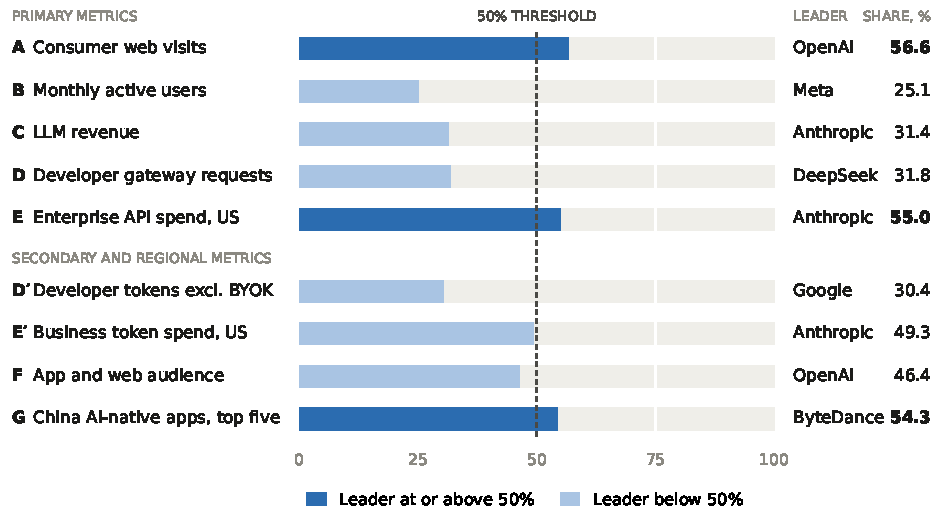
\includegraphics[width=\textwidth]{figs/fig_leader.pdf}
\caption{Share of the leading vendor in each metric. Dark bars: leader at or above the 50\% threshold (three of nine). The identity of the leader changes with the unit of measurement.}
\label{fig:leader}
\end{figure}

Table~\ref{tab:conc} and Figure~\ref{fig:leader} give the first result, and it cuts against a naive reading of our title. Every metric is at least moderately concentrated, and six of nine exceed an HHI of 1{,}800. Local dominance at $\tau=50$ is not rejected in three metrics: consumer web visits (OpenAI), US enterprise API spend (Anthropic) and Chinese AI-native apps (ByteDance). Two more leaders are above 40\% (E$'$, F). The weekly Ramp series shows Anthropic at 60.1\% of token spend in the week ending 11 October 2026 \cite{ramp2026index}, so E$'$ crosses the threshold in some weeks. Metrics A, F and G are computed over truncated sets of assistants, which biases their HHI upward relative to the full market. The $1/\mathrm{HHI}$ column restates each index as the number of equally sized firms that would produce it, which separates the metrics more legibly than the index does: consumer attention, enterprise spend and the Chinese app market run between 2.2 and 2.7 effective competitors, while developer volume and user reach run between 5.7 and 6.2. Two cautions apply to every row. The index is computed on one cross-section and says nothing about whether the positions hold: metric D is only moderately concentrated by the US bands and yet has three different leaders across the thirteen months of Section~\ref{sec:persist}, with 19.4\% of the market changing hands per month against 2.9\% for metric A, so two markets that the index places 1.5 effective competitors apart differ by a factor of seven in turnover. The index also presumes that a share measures power, which multi-homing weakens (Section~\ref{sec:multihoming}). A leader below the threshold does not by itself reject the local null. Under the error model of rule 6 the one-dimensional test rejects at the 5\% level only when the leader holds less than 28.1\%, and that happens in one of the nine metrics (B, Meta at 25.1\%, $p=0.024$). For C, D and D$'$ the leader holds between 30\% and 32\% and $p$ lies between 0.08 and 0.10; for E$'$ and F it exceeds 0.4. On point estimates local dominance appears in three metrics; under the error model it is excluded in one. Section~\ref{sec:markets} asks whether the three local dominances survive a second source.

\subsection{Market-level tests with second sources}
\label{sec:markets}

\begin{table}[t]
\centering\footnotesize
\caption{Local null by candidate relevant market, with every reading found. Share: leader's share (\%). ``Interest'' marks a publisher with a stake in one of the vendors.}
\label{tab:markets}
\begin{tabularx}{\textwidth}{@{}L{3.8cm} X l r@{}}
\toprule
Market & Reading & Leader & Share \\
\midrule
M1 Consumer assistants & Similarweb web visits, seven assistants, Oct 2026 \cite{momentic2026chatbots} & OpenAI & 56.6 \\
outside China & StatCounter page views, Oct 2026 \cite{statcounter2026} & OpenAI & 51.6 \\
 & StatCounter page views, Aug 2026 \cite{statcounter2026} & OpenAI & 79.4 \\
 & Sensor Tower app and web audience, May 2026 \cite{sensortower2026state} & OpenAI & 46.4 \\
\addlinespace
M2 Enterprise model & Menlo survey, US, 2026; interest: Anthropic \cite{menlo2026state} & Anthropic & 55.0 \\
spend & Ramp transactions, US, Oct 2026 \cite{ramp2026index} & Anthropic & 49.3 \\
 & Ramp transactions, US, week to 15 Nov 2026 \cite{ramp2026index} & Anthropic & 58.7 \\
 & Moss card spend, Europe, Jan 2024--May 2026 \cite{moss2026spend} & Anthropic & 52.8 \\
 & a16z survey, Global 2000 CIOs, Jan 2026; interest: OpenAI \cite{a16z2026cio} & OpenAI & 56 \\
\addlinespace
M3 Developer inference & OpenRouter requests by model author, Nov 2026 \cite{openrouter2026rankings} & DeepSeek & 31.8 \\
through gateways & OpenRouter paid tokens by author, Oct 2026 \cite{aimultiple2026share} & Google & 30.4 \\
 & Requests by seller, reconstructed, Nov 2026 (Section~\ref{sec:vendor}) & OpenAI & 19.0 \\
\addlinespace
M4 Consumer AI apps & QuestMobile, five largest AI-native apps, Sep 2026 \cite{questmobile2026q3} & ByteDance & 54.3 \\
in China & AICPB, five largest Chinese assistants by firm, Jun 2026 \cite{aicpb2026june} & Alibaba & 42.0 \\
 & AICPB, the same without Quark, Jun 2026 \cite{aicpb2026june} & ByteDance & 39.6 \\
\bottomrule
\end{tabularx}
\end{table}

Table~\ref{tab:markets} applies the local null to the four candidate markets of Section~\ref{sec:entities}. Each of the three local dominances of Table~\ref{tab:conc} rested on one source. With second sources the picture changes in every case.

\paragraph{M1, consumer assistants outside China.} All four readings name OpenAI and three place it at or above 50\%. StatCounter's worldwide figure for ChatGPT fell from 79.4\% in August 2026 to 51.6\% in October while Perplexity rose from 4.3\% to 15.0\% on the same tracker \cite{statcounter2026}. Similarweb shows no comparable movement, and we cannot tell whether the market or the tracker changed. By region, StatCounter places ChatGPT first in five of six regions and at or above 50\% in three: Asia (55.8\%), North America (74.2\%, September) and Oceania (70.2\%, July). It is below 50\% in Africa (45.9\%, with Gemini at 39.0\%) and in Europe (43.4\% against 38.6\%), and Gemini leads South America with 49.3\% against 37.1\%. This is the only source we found that covers Africa, and it counts page views referred by chatbots and not users. At world level the leader is at or above 50\% on both trackers. In three of six regions it is below 50\%, by margins (43\% to 49\%) that the error model cannot distinguish from 50\% ($p$ between 0.34 and 0.48).

\paragraph{M2, enterprise model spend.} The five readings all show a leader between 49\% and 59\%, and four show one at or above 50\%. They disagree on who it is. Menlo Ventures, an investor in Anthropic, reports Anthropic at 55\% of US enterprise API spend \cite{menlo2026state}. Andreessen Horowitz, an investor in OpenAI, reports OpenAI at about 56\% of model spend among 100 Global 2000 CIOs, with OpenAI models in production at 78\% of those firms and Anthropic's at 44\% \cite{a16z2026cio}. The two sources compiled from transactions side with the first. Anthropic took 49.3\% of US business token spend in October and 58.7\% in the week to 15 November \cite{ramp2026index}, and 52.8\% of card spend on AI tools among European customers of one spend-management firm, against 38.5\% for OpenAI, although OpenAI was bought by more of those companies (73.2\% against 68.1\%) \cite{moss2026spend}. The a16z survey is the earliest of the five readings and covers the largest firms. Our reading is that M2 has a firm at or near a majority of spend, that the weight of the evidence in late 2026 names Anthropic, and that the identity of the leader is not robust to the source. The Moss data extend the finding from the United States to Europe.

\paragraph{M3, developer inference through gateways.} Three readings give three leaders: DeepSeek by requests attributed to the model author, Google by paid tokens, and OpenAI when requests are attributed to the seller. None is above 32\%. Under the error model only the seller-based reading rejects the local null ($p=0.003$); the two author-based readings give $p=0.10$ and $p=0.08$. The stronger evidence against a dominant firm in this market is the turnover of its leader (Section~\ref{sec:persist}).

\paragraph{M4, consumer AI applications in China.} QuestMobile gives ByteDance 54.3\% of the monthly users of the five largest AI-native apps. A second panel, the AICPB ranking for June 2026, lists Doubao at 324 million monthly users, Qwen at 251 million, Quark at 159 million, DeepSeek at 139 million and Yuanbao at 104 million \cite{aicpb2026june}. Doubao has 33.2\% of these five and Alibaba's two applications 42.0\%; without Quark, which is an AI browser and search application, Doubao has 39.6\%. The leader is above 50\% on one panel and below it on the other, and the lower readings do not reject the local null under the error model ($p$ between 0.25 and 0.31). The panels differ in month, in geography (China against worldwide users of Chinese apps) and in the set of applications, and neither documents its method in a form we could audit.

\paragraph{Summary.} On point estimates, the first local dominance (M1) is confirmed by a second tracker at world level and not in every region; the second (M2) is confirmed as a property of the market and not of a particular firm; the third (M4) is not confirmed. Under the error model none of the readings below 50\% in M1, M2 or M4 excludes dominance. The second sources therefore weaken the identification of a dominant firm without establishing that there is none. A market-level statement of dominance has to name its source as well as its unit.


\subsection{Vendor level: the universal test}
\label{sec:vendor}

\begin{table}[t]
\centering\small
\caption{Vendor shares (\%) in the five primary dimensions. Bold marks the leader of each dimension. Notes: A uses the by-lab series of \cite{aimultiple2026share}; Anthropic's MAU uses a Q1 2026 estimate of 134 million; Meta is unlisted in D (below 1.6\%, set to 0.8); open-source models hold 4\% of E in total, split evenly here.}
\label{tab:matrix}
\begin{tabular}{@{}lrrrrrrrr@{}}
\toprule
& A & B & C & D & E & $\min_d$ & $\kappa(50)$ & dims $\ge50$ \\
\midrule
OpenAI & \textbf{56.2} & 20.9 & 29.0 & 19.0 & 31.0 & 19.0 & 2.6 & 1 \\
Google & 24.6 & 20.9 & 12.1 & 15.1 & 9.0 & 9.0 & 5.6 & 0 \\
Anthropic & 11.7 & 2.8 & \textbf{31.4} & 6.3 & \textbf{55.0} & 2.8 & 17.9 & 1 \\
DeepSeek & 3.3 & 3.0 & 0.2 & \textbf{31.8} & 1.3 & 0.2 & 250 & 0 \\
Meta & 0.5 & \textbf{25.1} & 1.4 & 0.8 & 1.3 & 0.5 & 100 & 0 \\
Alibaba & 0.3 & 6.7 & 2.9 & 6.2 & 1.3 & 0.3 & 161 & 0 \\
\bottomrule
\end{tabular}
\end{table}

Table~\ref{tab:matrix} and Figure~\ref{fig:heatmap} give the cross-dimension matrix. No vendor reaches 50\% in more than one of five dimensions. Four distinct vendors lead the five dimensions (OpenAI, Meta, Anthropic, DeepSeek). Three of these leads are robust (lead ratio $\ge1.5$: OpenAI in A, DeepSeek in D, Anthropic in E) and two are fragile (Meta in B at 1.20, Anthropic in C at 1.08); restricting attention to robust leads still yields three different leaders. Every vendor has $\kappa_v(50)>2$, so rule 2 rejects $\Hzero(50)$ for every vendor; the calibrated test below attaches an error rate to that verdict.

\begin{figure}[t]
\centering
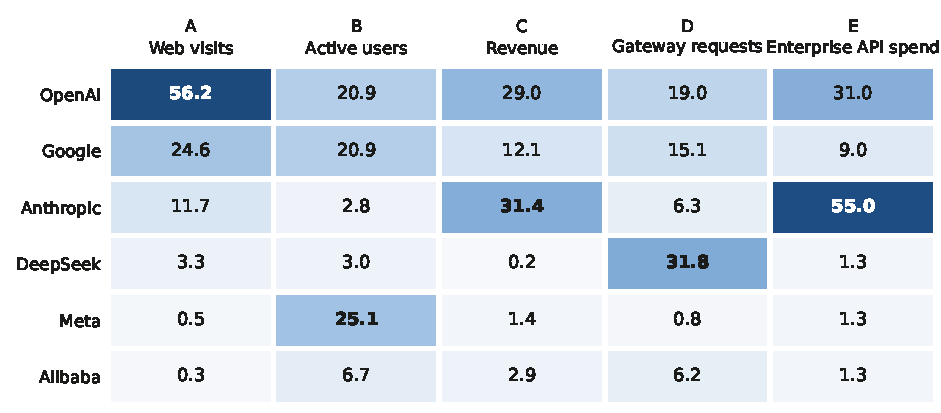
\includegraphics[width=\textwidth]{figs/fig_heatmap.pdf}
\caption{Vendor shares (\%) by dimension (primary matrix of Table~\ref{tab:matrix}). Bold marks the leader of each column. Universal dominance would appear as one uniformly dark row.}
\label{fig:heatmap}
\end{figure}

\begin{table}[t]
\centering\small
\caption{Sensitivity analysis most favourable to $\Hzero$: each cell is the largest share (\%) reported by any source for that vendor and dimension. $\kappa$: factor of understatement required in the weakest dimension; ``fail'': number of dimensions below $\tau$. OpenAI's value in A is StatCounter's share for August 2026 \cite{statcounter2026} and its value in E is the wallet share reported by a16z \cite{a16z2026cio}.}
\label{tab:fav}
\begin{tabular}{@{}lrrrrrrrrrrr@{}}
\toprule
& A & B & C & D & E & $\kappa(50)$ & fail & $\kappa(40)$ & fail & $\kappa(30)$ & fail \\
\midrule
OpenAI & 79.4 & 46.4 & 29.0 & 22.5 & 56.0 & 2.23 & 3 & 1.78 & 2 & 1.34 & 2 \\
Google & 24.7 & 27.7 & 12.1 & 30.4 & 9.0 & 5.56 & 5 & 4.44 & 5 & 3.33 & 4 \\
Anthropic & 11.7 & 10.3 & 31.4 & 9.8 & 58.7 & 5.10 & 4 & 4.08 & 4 & 3.06 & 3 \\
DeepSeek & 3.5 & 3.0 & 0.2 & 31.8 & 4.0 & 250 & 5 & 200 & 5 & 150 & 4 \\
Meta & 0.5 & 25.1 & 1.4 & 1.8 & 4.0 & 100 & 5 & 80 & 5 & 60 & 5 \\
\bottomrule
\end{tabular}
\end{table}

Table~\ref{tab:fav} repeats the test on the matrix most favourable to the null. At $\tau=50$ rule 2 rejects for every vendor: OpenAI, the closest case, would need its developer share to be understated by a factor of 2.23 and, simultaneously, its revenue share by a factor of 1.72. At $\tau=40$ OpenAI's margin falls to 1.78, inside the tolerance band, with two dimensions still below threshold; we classify this as rejected for all other vendors and inconclusive for OpenAI. At $\tau=30$ OpenAI is within a factor of 1.34 (developer) and 1.03 (revenue) of satisfying the null in all five dimensions. \emph{At the 30\% level the data cannot exclude that OpenAI holds a substantial share everywhere.} The claim of this paper is therefore specific to dominance in the legal sense of a majority or near-majority share.

\paragraph{Measurement-error simulation.} Figure~\ref{fig:mc} gives the share of simulated draws in which the null holds. At the reference error scale ($\sigma=0.35$), $\Hzero(50)$ holds in 0.02\% of draws with independent errors and 0.37\% with errors correlated within vendor; $\Hzero(40)$ in 0.5\% and 2.7\%; $\Hzero(30)$ in 8.2\% and 15.1\%. On the primary matrix the three figures are 0\%, 0\% and 0.4\%. With correlated errors $\Hzero(50)$ reaches 5\% of draws only at $\sigma=0.70$, where 95\% of errors lie within a factor of 3.9, and $\Hzero(40)$ at $\sigma=0.45$ (a factor of 2.4). These are plug-in quantities. They start from the observed shares and ask how often noise would lift them above the threshold; they are not the error rates of a test, and they overstate the evidence against the null.

\begin{figure}[t]
\centering
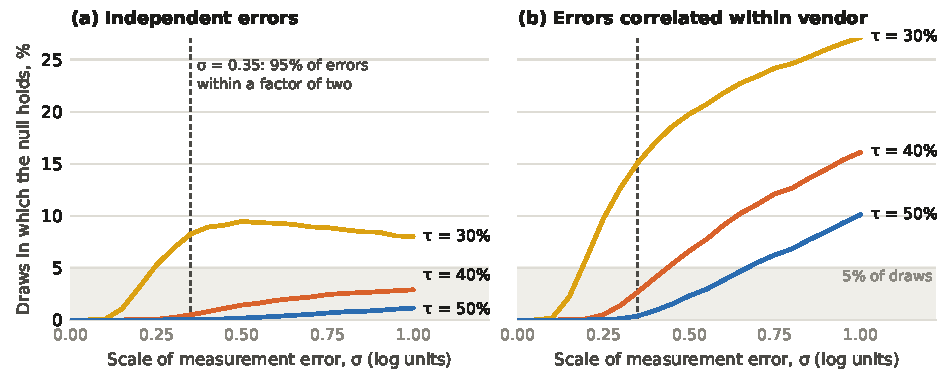
\includegraphics[width=\textwidth]{figs/fig_mc.pdf}
\caption{Share of 100{,}000 simulated draws in which universal dominance holds for some vendor, as a function of the scale of multiplicative measurement error, on the matrix most favourable to $\Hzero$. Shaded band: below 5\%. Dashed line: $\sigma=0.35$.}
\label{fig:mc}
\end{figure}

\paragraph{Calibrated test and error rates.} Rule 2 with $\kappa^{*}=2$ rejects a vendor that truly holds 50\% in every dimension with probability 0.1\% when $\sigma=0.2$, 11\% when $\sigma=0.35$ and 35\% when $\sigma=0.5$; a 5\% rate at $\sigma=0.35$ requires $\kappa^{*}=2.25$. OpenAI's margin of 2.63 on the primary matrix clears that value and its margin of 2.23 on the most favourable matrix does not. Table~\ref{tab:pooled} gives the pooled test of rule 7 for the best-placed entity in each specification. On single-source data $\Hzero(50)$ is rejected at the 5\% level under both error structures ($p=0.0002$ and $p=0.018$) and at the larger error scale $\sigma=0.5$ ($p=0.009$). The rejection holds at the 5\% level for any error scale up to $\sigma=0.65$ with independent errors (95\% of errors within a factor of 3.6) and up to $\sigma=0.45$ with correlated errors (a factor of 2.4). $\Hzero(40)$ is rejected with independent errors ($p=0.010$) and not with correlated errors ($p=0.076$). $\Hzero(30)$ is not rejected. On the matrix most favourable to the null, $\Hzero(50)$ is not rejected ($p=0.07$ with independent errors, $0.16$ with correlated errors). That matrix is a biased selection, because it takes the largest value among sources in every cell, and a test applied to it is conservative. The result nevertheless shows where the conclusion depends on the choice of source: StatCounter's August reading in A, the app-and-web audience in B and the a16z survey in E. We therefore state the result in two parts. Universal dominance at 50\% is rejected on single-source data, and it is not excluded when every disagreement between sources is resolved in favour of the null.

\begin{table}[t]
\centering\small
\caption{Pooled shortfall test (rule 7) for the best-placed entity, $\sigma=0.35$. $T$: observed statistic at $\tau=50$. $p$-values at the least favourable point of the null, with independent errors and with errors sharing half of their variance within the entity ($\rho=0.5$). Blocs are defined in Section~\ref{sec:blocs}.}
\label{tab:pooled}
\begin{tabular}{@{}lrrrrrr@{}}
\toprule
& & \multicolumn{2}{c}{$\tau=50$} & \multicolumn{2}{c}{$\tau=40$} & $\tau=30$ \\
\cmidrule(lr){3-4}\cmidrule(lr){5-6}\cmidrule(lr){7-7}
Specification (entity) & $T$ & indep. & $\rho=0.5$ & indep. & $\rho=0.5$ & indep. \\
\midrule
Primary matrix (OpenAI) & 2.86 & 0.0002 & 0.018 & 0.010 & 0.076 & 0.33 \\
Common denominator (OpenAI) & 2.13 & 0.006 & 0.060 & 0.129 & 0.203 & 0.75 \\
Most favourable matrix (OpenAI) & 1.42 & 0.074 & 0.161 & 0.301 & 0.304 & 0.77 \\
Bloc OpenAI+Microsoft, primary & 2.21 & 0.004 & 0.053 & 0.102 & 0.184 & 0.72 \\
Bloc OpenAI+Microsoft, most favourable & 1.13 & 0.172 & 0.231 & 0.528 & 0.424 & 0.85 \\
Bloc Google+Anthropic, primary & 2.06 & 0.007 & 0.067 & 0.124 & 0.200 & 0.56 \\
Bloc Google+Anthropic, most favourable & 0.95 & 0.268 & 0.287 & 0.900 & 0.713 & 1.00 \\
\bottomrule
\end{tabular}
\end{table}

\paragraph{Dimension D by seller.} Section~\ref{sec:openseg} shows that the lab which releases open weights serves only part of the tokens of its models: 14\% for DeepSeek, 51\% for Qwen and 8\% for Zhipu's GLM. Applying those fractions to the requests of dimension D gives seller shares of 19.0\% for OpenAI, 15.1\% for Google, 6.3\% for Anthropic, 4.5\% for DeepSeek and 3.2\% for Alibaba. The figures for the closed labs are upper bounds, since cloud resellers also serve their models. With the seller as the unit, the leader of D is OpenAI and the five dimensions have three distinct leaders in place of four (OpenAI in A and D, Meta in B, Anthropic in C and E). OpenAI's weakest share and its margin are unchanged. Rank concordance rises from $W=0.379$ ($p=0.079$) to $W=0.525$ ($p=0.010$): counted by seller, the ordering of vendors is more consistent across dimensions and can be distinguished from no concordance. The count of four leaders and the weak concordance of the primary specification therefore owe part of their size to the unit used in D, and we report both readings.

\paragraph{Common denominator.} When each dimension is renormalised over the six vendors of the matrix, all shares rise. OpenAI's weakest share becomes 24.0\% (D), its margin falls to 2.08 and the pooled test gives $p=0.006$ with independent errors and $p=0.060$ with correlated errors. The leaders of the five dimensions do not change.

\paragraph{Rank concordance.} For six vendors and five dimensions, $W=0.379$ (permutation $p=0.079$). For the four vendors present in all sources (OpenAI, Google, Anthropic, DeepSeek), $W=0.233$ ($p=0.35$); adding the three secondary metrics gives $W=0.343$ ($p=0.035$, eight metrics that are not independent). Concordance is far from the value of 1 implied by a stable hierarchy and, in the primary specification, is not distinguishable from no concordance. One regularity survives: among the four, OpenAI is never ranked below second in any primary dimension (mean rank 1.7), while Anthropic and DeepSeek each range from first to fourth. OpenAI is pervasive without being dominant.

\subsection{Ownership blocs and vertical ties}
\label{sec:blocs}

The tests above treat each lab as an independent firm. Two of the leading vendors are partly owned by their largest distributors. Microsoft held about 27\% of OpenAI after the 2025 recapitalisation and about 24\% on an as-converted basis in September 2026, according to summaries of its quarterly filing; OpenAI pays Microsoft a share of revenue until 2030, and the exclusivity of Azure ended in April 2026 \cite{microsoft2026q1,cnbc2026openai}. Anthropic listed its shares on 19 November 2026. After the offering Amazon holds 14.7\% and Google 13.7\% of its capital in non-voting stock, Microsoft and NVIDIA bought shares in a concurrent placement, and about 47\% of its 2025 revenue came through cloud marketplaces \cite{fortune2026anthropic,csa2026frontier}. The filing, as quoted in \cite{fortune2026anthropic}, says that these partners ``simultaneously serve as our investors, customers, distribution partners, and competitors''.

\begin{table}[t]
\centering\small
\caption{Universal test with vendors linked by equity counted as one entity. Shares in \%. In B, Microsoft's unlisted user base is set to the whole unattributed residual of the source, an upper bound. ``Fail'': dimensions below 30\%.}
\label{tab:blocs}
\begin{tabular}{@{}llrrrrrrr@{}}
\toprule
Entity & Matrix & A & B & C & D & E & $\kappa(50)$ & fail(30) \\
\midrule
OpenAI & primary & 56.2 & 20.9 & 29.0 & 19.0 & 31.0 & 2.63 & 3 \\
 & most favourable & 79.4 & 46.4 & 29.0 & 22.5 & 56.0 & 2.23 & 2 \\
OpenAI+Microsoft & primary & 56.9 & 29.8 & 36.2 & 20.6 & 31.0 & 2.43 & 2 \\
 & most favourable & 82.2 & 46.4 & 36.2 & 24.1 & 56.0 & 2.08 & 1 \\
Google+Anthropic & primary & 36.3 & 23.7 & 43.5 & 21.4 & 64.0 & 2.34 & 2 \\
 & most favourable & 36.4 & 38.0 & 43.5 & 40.2 & 64.0 & 1.37 & 0 \\
\bottomrule
\end{tabular}
\end{table}

Table~\ref{tab:blocs} repeats the universal test under the extreme assumption that each stake makes the two firms one entity. On single-source data the rejection of $\Hzero(50)$ survives: the margin is at least 2.34 for either bloc, and the pooled test gives $p=0.004$ and $p=0.007$ with independent errors, although it is no longer below 5\% with correlated errors ($p=0.053$ and $0.067$; Table~\ref{tab:pooled}). On the most favourable matrix the result changes. A Google--Anthropic bloc holds at least 36.4\% in every dimension, so $\Hzero(30)$ is satisfied outright, $\Hzero(40)$ fails in two dimensions by a factor of 1.10, and $\Hzero(50)$ cannot be rejected ($p=0.27$). Whether Google and Anthropic are one entity is the assumption to which the universal result is most sensitive.

The assumption is far from the facts. Google's stake is 13.7\%, carries no votes, and sits beside a larger stake held by Amazon; Gemini and Claude compete in every dimension measured here. The partial-ownership adjustment of rule 8 gives the size of the effect under a silent financial interest. It adds 49 points to the HHI of A, 102 to C and 68 to E, against 657, 1{,}177 and 990 for a full merger. The stakes do not make the labs one firm. They do mean that the vendor shares of Table~\ref{tab:matrix} understate the common interests among the firms listed, by an amount that lies between those two columns, and that the three largest cloud providers, which together hold 61\% of cloud infrastructure (Section~\ref{sec:upstream}), are shareholders of the two leading model vendors and the main resale channel for their models.

\subsection{Paradigm level: closed versus open weights}
\label{sec:paradigm}

\begin{figure}[t]
\centering
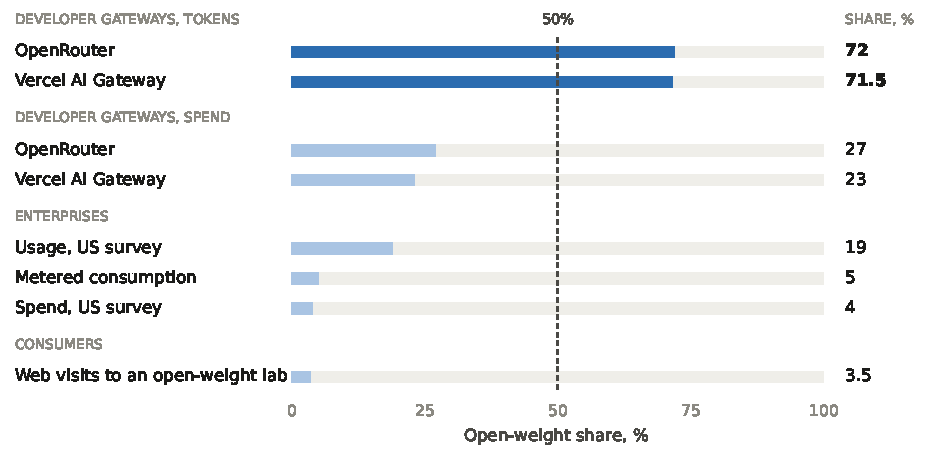
\includegraphics[width=\textwidth]{figs/fig_open.pdf}
\caption{Open-weight share in eight metrics (September--October 2026). Open-weight models exceed 50\% only in gateway token volume.}
\label{fig:open}
\end{figure}

Figure~\ref{fig:open} shows the open-weight share in eight metrics. It ranges from 3.5\% to 72\%. Open weights exceed 50\% in two metrics, both gateway token volume: 72\% on OpenRouter in the latest week reported \cite{openrouter2026tokens} and 71.5\% on Vercel's gateway \cite{vercel2026index}. Closed weights exceed 50\% in the other six: gateway spend (73\% on OpenRouter, 77\% on Vercel), US enterprise usage (81\%) and spend (96\%) \cite{menlo2026state}, enterprise metered consumption (about 95\%) \cite{futurum2026open} and consumer web visits (96.5\% among seven assistants). On point estimates neither paradigm satisfies $\Hzero(50)$: the open-weight side is below 50\% in six of eight metrics and the closed-weight side in two. Under the rules of Section~\ref{sec:rules} the two sides are not in the same position. Dominance by open weights is rejected ($\kappa=14.3$; pooled $p<10^{-4}$). Dominance by closed weights is not. Its weakest share is 28.0\%, so $\kappa=1.79$ lies inside the tolerance band, and the pooled test gives $p=0.44$ with the eight metrics taken as independent and $p=0.56$ when they are grouped into five (gateway tokens, gateway spend, enterprise usage, enterprise spend, consumer visits). The only evidence against closed-weight dominance is the token count of two gateways, and an understatement of the closed share there by a factor of 1.8 would remove it.

Scale points the same way. OpenRouter routed 128.4 trillion tokens in the week of 14 September 2026 \cite{openrouter2026tokens}, about 18.3 trillion per day. ByteDance alone reported 180 trillion tokens per day for its Doubao models in June 2026 \cite{tmtpost2026doubao}, and Google reported 3.2 quadrillion tokens per month across its surfaces in May 2026 \cite{register2026io}, about 107 trillion per day. The gateway is about 6\% of the sum of those two closed-weight providers (Figure~\ref{fig:scale}). If metrics were weighted by volume, the two metrics in which open weights lead would carry little weight, and closed-weight dominance could not be excluded. We cannot compute that weighted share because no source reports global tokens by paradigm.

\begin{figure}[t]
\centering
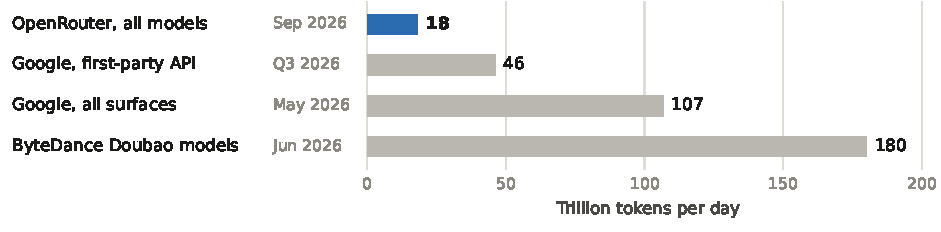
\includegraphics[width=\textwidth]{figs/fig_scale.pdf}
\caption{Daily token volume of the largest neutral gateway against three first-party figures (company disclosures, different months in 2026). Google's API figure is 32 billion tokens per minute converted to a day \cite{alphabet2026q3}.}
\label{fig:scale}
\end{figure}

The token and spend metrics are consistent once price is considered. With open-weight shares $t$ of tokens and $s$ of spend, the implied closed-to-open price ratio is $[t/(1-t)]/[s/(1-s)]$: 7.0 on OpenRouter and 8.4 on Vercel. This agrees with the sixfold gap measured in 2025 \cite{nagle2025latent}, with Vercel's statement that open-weight models sold at about a seventh of frontier rates \cite{vercel2026open}, and with the 90\% discount for comparable intelligence reported by Demirer et al.\ \cite{demirer2026emerging}. Token share and spend share therefore describe one market at two price levels and do not conflict. With a short-run price elasticity just above one \cite{demirer2025emerging}, a lower price raises volume roughly in proportion and leaves spend about unchanged, which is what the two series show.

Three further facts qualify the paradigm reading. First, the open-weight token lead is recent and price-sensitive: closed models held about 80\% of tokens on the same platform in 2025 \cite{nagle2025latent}; Xiaomi's share of paid developer tokens went from 2.8\% (May 2026) to 70.34\% (July) and 8.12\% (October) \cite{aimultiple2026share}. Second, on Vercel one model, DeepSeek V4.1 Flash, processed nearly half of September tokens for 2.6\% of spend \cite{vercel2026index}. Third, in enterprises ``open'' does not mean ``Chinese'': among 83 production users surveyed by Futurum the most used families were Google Gemma (55\%), Microsoft Phi (39\%), Meta Llama (35\%), DeepSeek (25\%), NVIDIA Nemotron (25\%), Mistral (24\%), Alibaba Qwen (10\%), Moonshot Kimi (6\%) and Zhipu GLM (1\%); 42\% of 200 enterprises ran open weights in production and origin was a major or deciding factor for 47\% of production users \cite{futurum2026open}. The pattern is not specific to North America: in a 2025 survey of more than 700 technology leaders in 41 countries, 63\% of organisations used an open-source AI model and 76\% expected to use more, while 56\% named security and compliance and 45\% long-term support as barriers \cite{mckinsey2025open}. Open weights are thus present in most organisations and absent from most of the bill.

Open-weight volume is also concentrated. DeepSeek alone accounts for 62.5\% of the tokens of the ten most used models on OpenRouter \cite{openrouter2026rankings}, and the leading open families in enterprises belong to Google, Microsoft, Meta and NVIDIA. This matches the argument that openness does not by itself disperse market power \cite{widder2024open} and the prediction that an open ecosystem depends on large firms using openness strategically \cite{azoulay2025old}. Download activity is equally skewed \cite{osborne2024ai,hf2026summer}. A high open-weight share should therefore not be read as a deconcentrated market. Section~\ref{sec:openseg} examines the segment family by family.

\subsection{Origin level: US versus China}
\label{sec:origin}

\begin{table}[t]
\centering\small
\caption{Share (\%) of US-origin and China-origin labs. ``--'': not reported by the source. The country in \cite{aimultiple2026share} is that of the lab, not of the user.}
\label{tab:origin}
\begin{tabular}{@{}lrr@{}}
\toprule
Metric & US-origin & China-origin \\
\midrule
Consumer web visits, Oct 2026 \cite{aimultiple2026share} & 95.7 & 4.2 \\
Enterprise API spend, US, top three labs \cite{menlo2026state} & 95.0 & -- \\
LLM revenue, Q1 2026 \cite{counterpoint2026revenue} & 83.5 & 11.6 \\
Vendor MAU, Apr 2026 \cite{counterpoint2026mau} & 66.8 & 21.5 \\
Developer tokens excl.\ BYOK, Oct 2026 \cite{aimultiple2026share} & 65.3 & 29.2 \\
Developer tokens excl.\ BYOK, Jul 2026 \cite{aimultiple2026share} & 21.1 & 77.0 \\
Open-model downloads, Feb 2025--Feb 2026 \cite{hf2026spring} & 36.5 & 41.0 \\
Gateway tokens, Sep 2026 \cite{openrouter2026tokens} & -- & 69.0 \\
\bottomrule
\end{tabular}
\end{table}

Table~\ref{tab:origin} and Figure~\ref{fig:origin} give origin shares. US-origin labs exceed 50\% in five of the seven metrics that report a US figure; China-origin labs exceed 50\% in two of seven. On point estimates neither origin satisfies $\Hzero(50)$ across metrics, and the developer series reverses sign within three months (China 77.0\% in July, 29.2\% in October). Under the error model the two origins differ. Dominance by China-origin labs is rejected ($\kappa=11.9$; pooled $p<10^{-4}$). Dominance by US-origin labs is not rejected: with the latest reading of each metric the US share is below 50\% only in open-model downloads (36.5\%) and in gateway tokens (at most 31\%), so $\kappa=1.61$, and the pooled test gives $p=0.59$ with independent errors and $p=0.45$ with correlated errors. The asymmetry is nonetheless clear: US-origin labs hold a majority of every consumer and revenue metric outside China, and the Chinese lead is confined to gateway tokens and open-model downloads. Demand for those tokens is partly American: over 40\% of US startups on OpenRouter used DeepSeek in production in 2026, against about 13\% in January \cite{openrouter2026tokens}. Supply is partly American as well: more than half of the open-weight gateway tokens of Chinese families are sold by hosts headquartered in the United States (Section~\ref{sec:openseg}).

\begin{figure}[t]
\centering
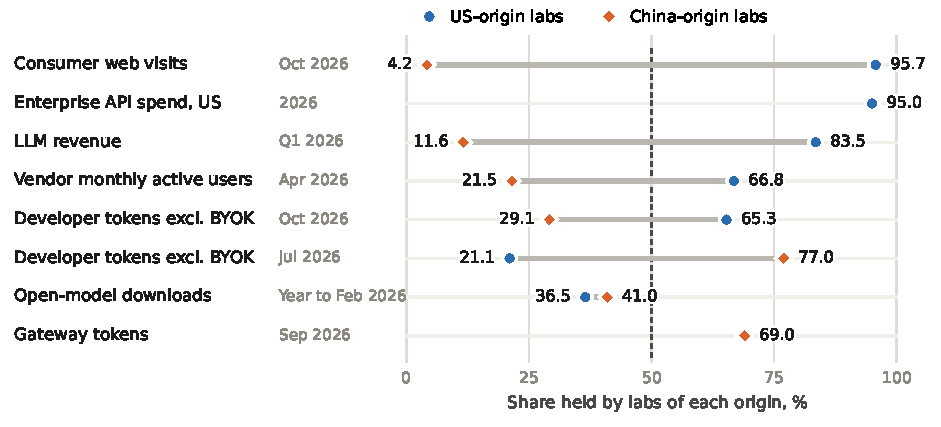
\includegraphics[width=\textwidth]{figs/fig_origin.pdf}
\caption{Share of US-origin and China-origin labs in eight metrics (values of Table~\ref{tab:origin}). Dashed line: 50\%. The side that leads depends on the metric, and the developer series reverses between July and October 2026.}
\label{fig:origin}
\end{figure}

\subsection{Inside the open-weight segment}
\label{sec:openseg}

The paradigm test treats open weights as one entity. This subsection opens that entity and repeats the test inside it, with model families as the entities and four layers of use as the dimensions: downloads from the Hugging Face Hub, local inference, tokens served through a public gateway, and production use in enterprises. Two of the sources used here have a stake in the result and one analysis is a reconstruction; Section~\ref{sec:validity} states the limits.

\begin{figure}[t]
\centering
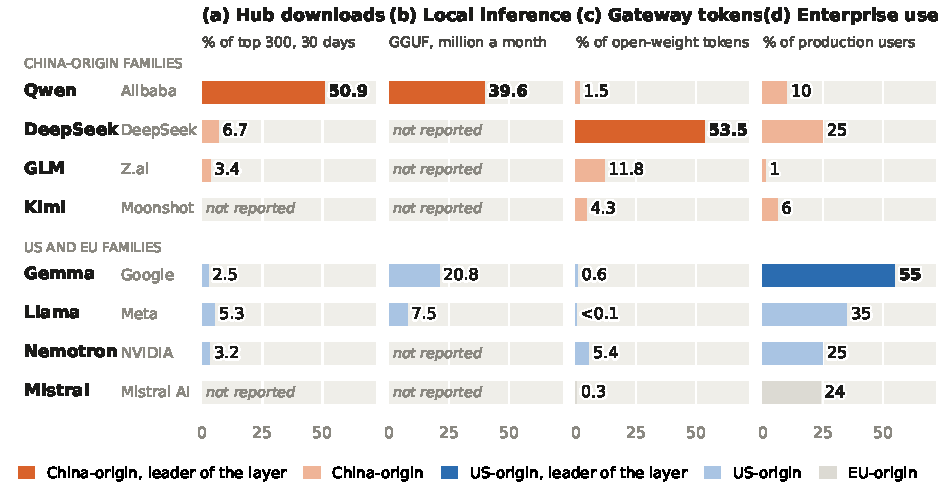
\includegraphics[width=\textwidth]{figs/fig_openfam.pdf}
\caption{Eight open-weight families in four layers of use. (a) Share of trailing 30-day downloads among the 300 most-downloaded text-generation repositories on the Hugging Face Hub, 4 November 2026 \cite{vidraft2026top300}. (b) Monthly downloads in GGUF, the format of local runtimes \cite{hf2026summer}. (c) Share of open-weight tokens on a large public router, 2--8 November 2026 \cite{amcompute2026providers}; Tencent's Hunyuan (12.4\%), not shown, is second. (d) Share of 83 enterprise production users running each family, several answers allowed \cite{futurum2026open}; Microsoft Phi (39\%), not shown, is second. Saturated bars mark the leader of each layer. Units differ between panels.}
\label{fig:openfam}
\end{figure}

\paragraph{The leading family depends on the layer.} Figure~\ref{fig:openfam} compares eight families. On the Hub, Qwen leads by a wide margin on every count: 50.9\% of trailing 30-day downloads among the 300 most-downloaded text-generation repositories on 4 November 2026, against 55.8\% on 17 September \cite{vidraft2026top300}; 46.3\% of the 2.04 billion cumulative downloads in the regional totals of the ATOM report to March 2026, about twice Llama's 23.4\% \cite{lambert2026atom}; 2.05 billion downloads in the first seven months of 2026; and 151{,}448 derivative repositories, 2.6 times Meta's total and 4.7 times Llama's, with Google second at 82{,}506 \cite{hf2026summer}. Qwen also leads local inference, with 39.6 million monthly downloads in the GGUF format against 20.8 million for Gemma and 7.5 million for Llama \cite{hf2026summer}. On the gateway the order is different. Of the open-weight tokens routed in the week of 2--8 November 2026, DeepSeek held 53.5\%, Tencent's Hunyuan 12.4\%, GLM 11.8\% and NVIDIA's Nemotron 5.4\%; Qwen held 1.5\% and Llama less than 0.1\% \cite{amcompute2026providers}. In enterprises the order changes again: the families most often in production were Gemma (55\% of users), Phi (39\%) and Llama (35\%), with Qwen at 10\% \cite{futurum2026open}. Three families lead the four layers, and the family that leads the Hub is fourth of six on the gateway and fifth of six in enterprises.

\paragraph{The test applied to families.} The decision rules of Section~\ref{sec:rules} give the same pattern for families as for vendors. Local dominance is not rejected in two layers: Qwen is at or above 50\% of 30-day Hub downloads in both snapshots (on the cumulative measure it is above 40\% and below 50\%), and DeepSeek exceeds 50\% of open-weight gateway tokens. Both layers are highly concentrated. The HHI of Hub downloads lies between 2{,}692 and 2{,}960 in November and between 3{,}220 and 3{,}388 in September, the lower figures excluding an architecture class (GPT/OPT, 15.4\%) that the source reports as one group although it is not one developer; the HHI of gateway tokens by family is 3{,}225 and the four largest families hold 83\%. Universal dominance is rejected: Qwen's weakest share is 1.5\% and DeepSeek's is 6.7\%, so the null would require understatement by factors of 33 and 7.5. For the six families observed in all of layers (a), (c) and (d), the rankings do not agree: Kendall's $W=0.141$ (permutation $p=0.87$). The rank correlation of Hub downloads with enterprise use is $-0.46$ and that of gateway tokens with enterprise use is $-0.61$; with six families neither can be distinguished from zero, and we report the signs only as description. The open-weight segment thus reproduces, one level down, the structure found for the whole market: each layer is concentrated, and the leader changes with the layer.

\paragraph{Two sub-ecosystems.} Model size explains the inversion. Models under one billion parameters take 83\% of all-time downloads and models above 70 billion took 3\% of downloads in 2026 \cite{hf2026summer}; in the ATOM data about three quarters of downloads are of models under 10 billion parameters, where Qwen holds 44\%, while DeepSeek holds 47\% of downloads above 250 billion \cite{lambert2026atom}. The share of each lab's 2026 downloads that went to models above 70 billion parameters was close to 100\% for MiniMax, 88\% for Moonshot, 55\% for DeepSeek and 39\% for Z.ai, against 14\% for NVIDIA, 9\% for Meta and about zero for Google, Microsoft and IBM \cite{hf2026summer}. The segment therefore has a small-model side, which is downloaded, fine-tuned and run locally or on premises (Qwen, Gemma, Llama, Phi), and a large-model side, which few users can host and which is consumed as hosted tokens (DeepSeek, GLM, Kimi, MiniMax, Hunyuan). The two sides differ in origin and in licence. China's largest open release of each month in 2026 had between 754 billion and 2.78 trillion parameters, while the largest US release stayed below 130 billion in five of seven months. Of 178 Chinese releases above 20 billion parameters, 59\% carried Apache 2.0 and 22\% MIT licences; of US releases in the same band, 29\% carried one of the two, 41\% custom terms and 30\% no declared licence. The direction is not fixed, since the two largest Chinese releases of mid-2026, Kimi K3 and a 2.4-trillion-parameter Qwen 3.8, added commercial restrictions \cite{hf2026summer}. Openness is a matter of degree along several dimensions \cite{liesenfeld2024rethinking}, which is a further reason not to read a two-way split of ``open'' against ``closed'' as a market share. Attention and use also diverge on the Hub: the 25 most downloaded and the 25 most liked repositories have one entry in common, none of the 25 most downloaded was published in 2026 and 13 date from 2022, and 85.6\% of models have fewer than 200 lifetime downloads \cite{hf2026summer}.

\begin{figure}[t]
\centering
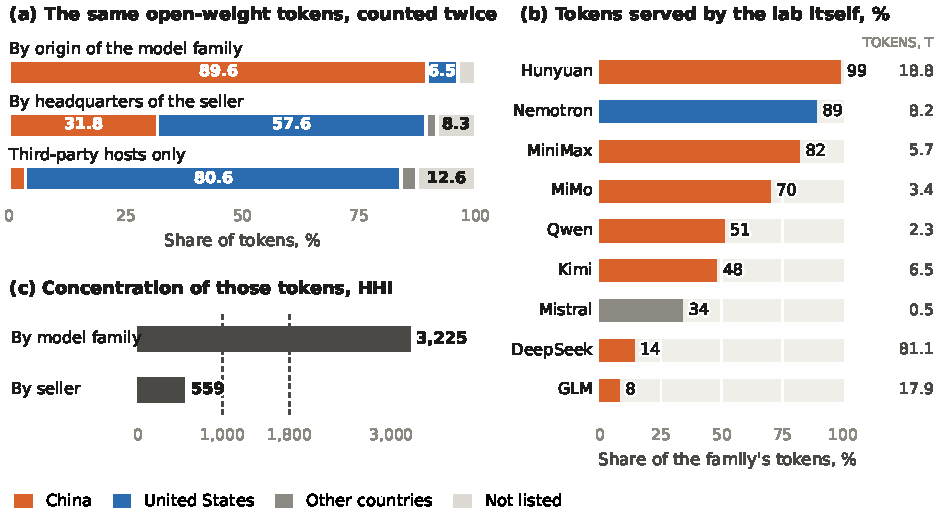
\includegraphics[width=\textwidth]{figs/fig_serving.pdf}
\caption{Open-weight tokens on a large public router, 2--8 November 2026 \cite{amcompute2026providers}. (a) The same tokens by origin of the model family, by headquarters of the firm that served them (lab APIs and third-party hosts together; our reconstruction) and for third-party hosts alone. ``Other countries'' are Singapore, the Netherlands, France, Indonesia and Sweden. (b) Share of each family's tokens served by the lab that built it, with weekly tokens in trillions; Gemma, gpt-oss and Llama have no lab API. (c) HHI of the same tokens with the family and with the seller as the unit; dashed lines at 1{,}000 and 1{,}800.}
\label{fig:serving}
\end{figure}

\paragraph{The author of the weights is not the seller of the tokens.} A closed model has one seller. An open-weight model can be served by anyone, and Figure~\ref{fig:serving} shows how far this goes. DeepSeek's own API served 14\% of the DeepSeek-family tokens on the router and Z.ai's served 8\% of GLM tokens, each family being offered by 46 providers; at the other extreme Tencent served 99\% of Hunyuan tokens, NVIDIA 89\% of Nemotron and MiniMax 82\% of its own \cite{amcompute2026providers}. Combining the family table and the provider table of that source, we estimate that labs served 35\% of open-weight tokens themselves and third-party hosts the remaining 65\%, with no host above 12.5\% of third-party volume. Counting sellers in place of families lowers the HHI of the same tokens from 3{,}225 to about 560; the largest single seller is Tencent's own service with 12.9\%, and DeepSeek as a firm sold about 8\% of the open-weight tokens of which its models were 53.5\%. Price does not settle the allocation: on the most used model DeepSeek served 20\% of tokens at \$0.60 per million output tokens while the cheapest listing, at \$0.15, served 0.5\% \cite{amcompute2026providers}.

The same substitution changes the origin reading. Families of Chinese origin account for 89.6\% of open-weight tokens on the router, but firms headquartered in China sold 31.8\% of them and firms headquartered in the United States 57.6\%; among third-party hosts the US share is 80.6\% and the Chinese share 3.4\%, or 7.1\% if Alibaba Cloud International, SiliconFlow and NovitaAI are counted as Chinese affiliates (Table~\ref{tab:openorigin}). Two consequences follow for the tests above. First, dimension D counts requests by model author. DeepSeek's 31.8\% of gateway requests (Table~\ref{tab:matrix}) is a share of authorship, and it overstates DeepSeek's position as a vendor in the one dimension that a China-origin lab leads. A firm that sells a minority of the tokens of its own models, in competition with dozens of hosts, is unlikely to have the ability to act independently of rivals and customers that the legal notion of dominance requires \cite{ec2009guidance}. Second, the 69\% of gateway tokens attributed to China-origin labs in Table~\ref{tab:origin} describes where the weights were trained. At least 54\% of the tokens of Chinese families were sold by US-headquartered hosts and 31.5\% by the labs themselves, so a large part of the corresponding revenue is earned outside China, although the source reports tokens and not dollars. This agrees with the finding that infrastructure sellers capture most of the value of enterprise open-weight use \cite{futurum2026open} and with the argument that open models leave control of compute where it was \cite{widder2024open}. Entry into serving is cheap and hosts are many, so this layer comes closer to a contestable market \cite{baumol1982contestable} than any other segment examined in this paper.

\begin{table}[t]
\centering\small
\caption{The open-weight segment by origin (\%). Origin is that of the lab that released the weights, except in the two rows on sellers. ``--'': not reported.}
\label{tab:openorigin}
\begin{tabular}{@{}lrr@{}}
\toprule
Measure & China & US \\
\midrule
Hub downloads, top 300 repositories, 30 days to 4 Nov 2026 \cite{vidraft2026top300} & 64.1 & 30.0 \\
Cumulative Hub downloads, Nov 2023--Mar 2026 \cite{lambert2026atom} & 56.5 & 35.5 \\
New derivative models, Feb 2026 \cite{lambert2026atom} & 70 & -- \\
Ten highest-scoring open models, Apr 2026 \cite{aa2026open} & 100 & 0 \\
Open-weight gateway tokens, by origin of the family \cite{amcompute2026providers} & 89.6 & 6.5 \\
The same tokens, by headquarters of the seller (reconstructed) & 31.8 & 57.6 \\
The same tokens, third-party hosts only \cite{amcompute2026providers} & 3.4 & 80.6 \\
\bottomrule
\end{tabular}
\end{table}

\begin{figure}[t]
\centering
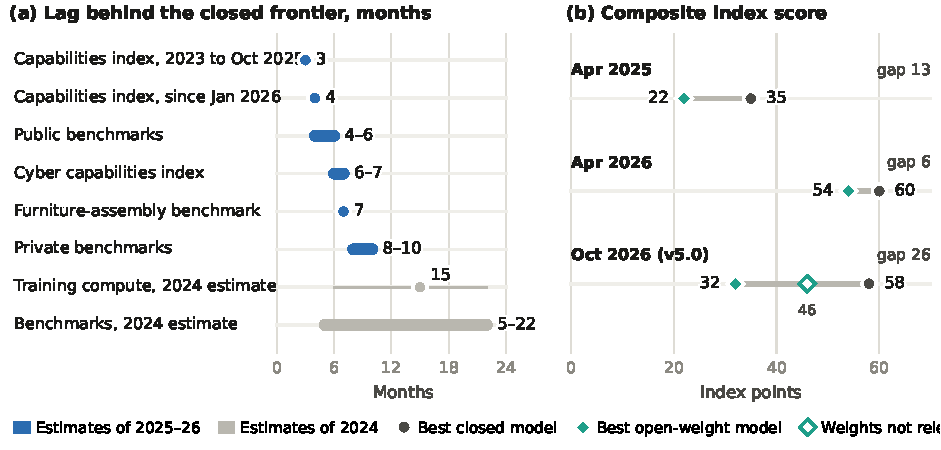
\includegraphics[width=\textwidth]{figs/fig_gap.pdf}
\caption{Distance between the best open-weight models and the closed frontier under different rulers. (a) Lag in months estimated by Epoch AI: aggregate capabilities index \cite{epoch2026gap}, public and private benchmarks \cite{epoch2026thread}, cyber and furniture-assembly evaluations \cite{epoch2026topics}, and the 2024 estimates for benchmarks (90\% interval) and training compute (point estimate, with the 90\% interval as a thin line) \cite{cottier2024far}. (b) Artificial Analysis Intelligence Index of the best closed and the best open-weight model at three dates \cite{aa2026open,implicator2026index}. The index was revised between dates, so scores are comparable within a row only; version 5.0 gives most of its weight to private test data.}
\label{fig:gap}
\end{figure}

\paragraph{How far behind the closed frontier.} The price advantage of open weights (Section~\ref{sec:paradigm}) is usually set against a capability gap, and that gap also depends on the ruler (Figure~\ref{fig:gap}). On Epoch AI's aggregate index the best open-weight models have trailed the closed frontier by four months, or eight index points, since January 2026, against three months between January 2023 and October 2025 \cite{epoch2026gap}; the 2024 estimate was about a year, with a 90\% interval of 5 to 22 months on benchmarks and a lag of 15 months in training compute \cite{cottier2024far}. The same organisation finds a gap of four to six months on public benchmarks and eight to ten on private ones \cite{epoch2026thread}, and six to seven months on cyber and visual-spatial evaluations \cite{epoch2026topics}. Artificial Analysis measured the best open-weight model 13 points behind the best closed model in April 2025 (22 against 35) and 6 points behind in April 2026 (54 against 60), when nine of the thirteen models on its intelligence-for-price frontier were open weights and the leading ones cost between one half and one sixth of comparable closed models \cite{aa2026open}. After the October 2026 revision of that index, which moved most of the weight to private test data, the best downloadable models scored 32 against 58, a gap of 26 points; one model whose weights had not been released went from 3 points behind the leader to 12 \cite{implicator2026index}. Scores from different versions cannot be chained, but both organisations find a gap about twice as large, or larger, when the test data are private. This is the pattern expected if public benchmarks are easier to optimise against \cite{bean2025measuring}, and it qualifies the statement that open weights have caught up. It also bears on origin: in April 2026 all ten highest-scoring open-weight models came from labs based in China, and the best from elsewhere were Gemma 4 and Nemotron 3 \cite{aa2026open}.

\paragraph{What this adds to the tests.} Three readings change. (i) Among open-weight families, as among vendors, no family dominates every layer, and each layer is highly concentrated. (ii) For open weights the entity ``vendor'' divides into an author and a seller. Shares by author, which is what gateways publish, measure which models are used; shares by seller measure who is paid. The first is concentrated and mostly Chinese, the second is dispersed and mostly American. Adding the seller count does not rescue $\Hzero$ at any level, since it lowers the largest share in dimension D, but it removes the main support for reading gateway tokens as evidence of Chinese market power. (iii) The capability gap that is supposed to explain why enterprises pay sevenfold for closed models was between 4 and 10 months, or between 6 and 26 points, during 2026 according to the ruler, so it cannot be used as a single explanatory number.

\subsection{User geography}
\label{sec:geo}

\paragraph{Assistant shares by country.} Among seven assistants tracked by Similarweb in 19 economies (Figure~\ref{fig:geo}; Appendix~\ref{app:geo}), ChatGPT leads in 17, Gemini in one (Italy, 44.8\% against 43.5\%) and DeepSeek in one (China, 73.2\%). ChatGPT is above 50\% in 12 of 19. Country HHIs range from 3{,}158 (Russia) to 5{,}707 (China), with a median of 4{,}458. In consumer web chat, then, local dominance holds in most countries measured; the lead is narrow (ratio below 1.2) only in Italy, Vietnam and Turkey. DeepSeek's share is 32.1\% in Russia and between 0.1\% and 2.6\% elsewhere outside China; it is 1.6\% in Brazil, where ChatGPT holds 65.1\%, Gemini 26.3\% and Claude 4.7\%. The Chinese figure covers only these seven assistants and excludes the domestic apps that lead the Chinese market. StatCounter's regional pages give a different picture for October 2026, with Gemini ahead of ChatGPT in South America (Section~\ref{sec:markets}); the two trackers measure different things and we do not reconcile them.

\begin{figure}[t]
\centering
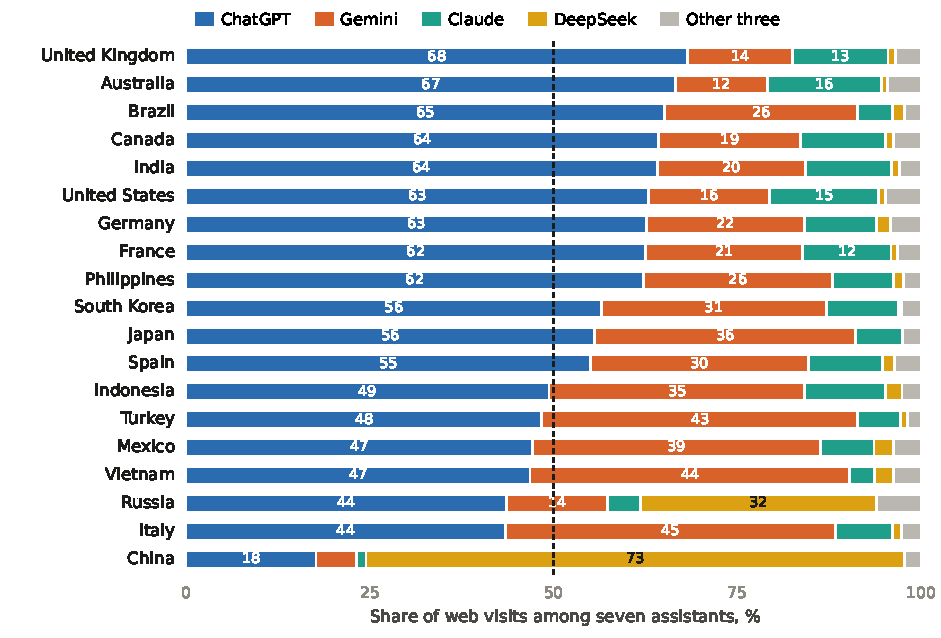
\includegraphics[width=\textwidth]{figs/fig_geo.pdf}
\caption{Composition of web visits among seven assistants by country, September 2026 (United States: October). Numbers are shares of 12\% or more. Dashed line: 50\%. The data cover only these seven assistants; values are in Appendix~\ref{app:geo}.}
\label{fig:geo}
\end{figure}

\paragraph{China as a separate market.} QuestMobile reports 546 million MAU for Chinese AI-native apps in September 2026, with Doubao at 419 million, Qwen at 158 million and DeepSeek at 123 million \cite{questmobile2026q3}. The CNNIC reports more than 700 million generative-AI users and penetration above 50\% by mid-2026, up from 602 million (42.8\%) at the end of 2025 \cite{cnnic2026genai}. None of the Western panels in Table~\ref{tab:data} observes this market.

\paragraph{Population-level adoption.} Microsoft estimates that 18.8\% of the world's working-age population used generative AI in Q2 2026: 28.8\% in the Global North and 16.2\% in the Global South, with the United Arab Emirates (73.3\%) and Singapore (64.3\%) at the top, the United States at 33.0\% (21st), Brazil at 20.2\%, India at 18.5\% and China at 17.5\% (67th) \cite{microsoft2026q2}. Surveys give higher levels: weekly use of standalone generative AI reached 51\% across six countries and 49\% in the United States in 2026, with ChatGPT at 34\%, Gemini at 24\%, Copilot at 11\% and Claude at 7\% \cite{reuters2026genai}. In Brazil, 32\% of internet users (about 50 million people) used generative AI in 2025, 69\% in class A against 16\% in classes D/E, and 59\% among those with higher education against 17\% with primary education ($n=24{,}535$) \cite{cetic2025tic}. Usage per capita correlates with income in every source that reports it \cite{misra2025measuring,anthropic2026index,liu2025who}. India became ChatGPT's largest market by weekly users in 2026 \cite{analytics2026india}, having reached 100 million weekly users in February \cite{techcrunch2026india}; a secondary compilation of Similarweb data puts the United States at 19.9\% of ChatGPT web traffic, India at 9.33\% and Brazil at 5.47\% \cite{elfsight2026chatgpt}. Users whose main language is not English are now over half of ChatGPT's active users, led by Spanish, Portuguese and Arabic \cite{openai2026expanded}. On the developer side the picture is inverted: by billing region, South America accounted for 1.21\% and Africa for 0.46\% of OpenRouter tokens in 2025, against 47.22\% for North America \cite{aubakirova2026state}.

\begin{figure}[t]
\centering
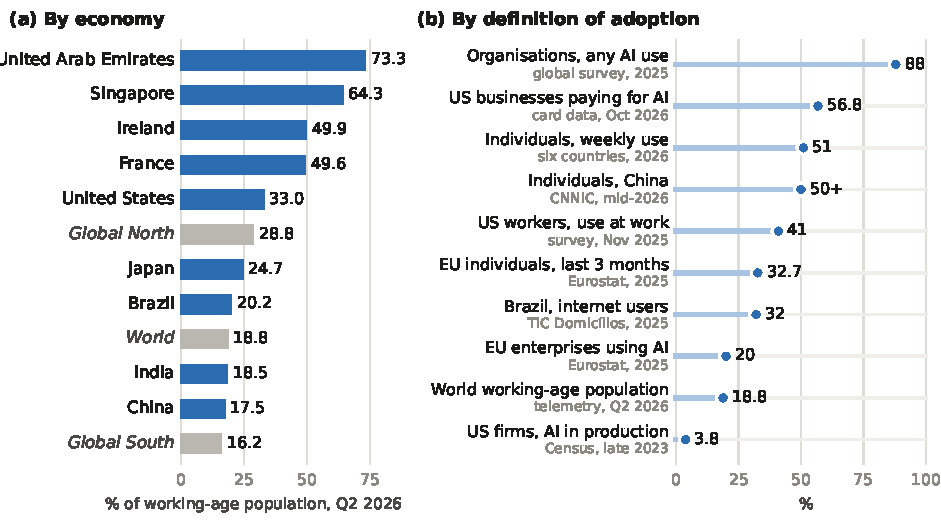
\includegraphics[width=\textwidth]{figs/fig_adoption.pdf}
\caption{Adoption of generative AI. (a) Share of the working-age population in selected economies, with aggregates in grey; Microsoft telemetry, Q2 2026 \cite{microsoft2026q2}. (b) Ten published answers to ``how many use AI?'', which differ in population, unit and definition (sources in the text).}
\label{fig:adoption}
\end{figure}

\paragraph{Adoption depends on the definition.} Published answers to ``how many use AI?'' range from 3.8\% to 88\% (Figure~\ref{fig:adoption}b). Some 88\% of organisations surveyed report some AI use \cite{aiindex2026}; 56.8\% of US businesses on one card platform pay for an AI product \cite{ramp2026index}; about 41\% of US workers report work-related use \cite{fed2026monitoring}; 32.7\% of EU individuals used generative AI in the previous three months, 64\% at ages 16--24 against 7\% at ages 65--74, and 20.0\% of EU enterprises use AI, up from 7.7\% in 2021 \cite{eurostat2025genai}; 3.8\% of US businesses used AI to produce goods and services in late 2023 \cite{census2023btos,bonney2024tracking}. The sensitivity to definition that this paper documents for market share applies equally to adoption itself. Vendor-agnostic measures point the same way: at least 13.5\% of 2024 biomedical abstracts show LLM processing \cite{kobak2025delving}.

\paragraph{Vendor user counts.} Reported user bases are large and not comparable: 1.2 billion weekly users for ChatGPT, stated by the company without a published methodology \cite{bigtech2026wau}; more than 1 billion monthly users for the Gemini app \cite{alphabet2026q3}; an estimated 1.2 billion monthly users for Meta AI \cite{counterpoint2026mau}; and panel estimates of 1.1 billion (ChatGPT), 662 million (Gemini) and 245 million (Claude) monthly users \cite{sensortower2026state}. Section~\ref{sec:validity} shows why these cannot be summed.

\subsection{Multi-homing}
\label{sec:multihoming}

Share measures implicitly assign one supplier to each user. Among weekly users in six countries, the four largest brands sum to 76\% against 51\% who use any tool \cite{reuters2026genai}, a lower bound of 1.49 tools per user. Multi-homing is common among apps on OpenRouter \cite{fradkin2025demand}. Firms behave differently: most concentrate their API usage on a single model even as the share trying several rises \cite{demirer2025emerging}. Because a share of multi-homing users implies less lock-in than the same share of exclusive users \cite{rochet2003platform,armstrong2006competition}, the 56.6\% of consumer web visits (A) overstates dependence on the leading assistant, whereas the enterprise spend share (E) is closer to a measure of dependence.

\paragraph{Concentration net of multi-homing.} The difference can be put in the units of Section~\ref{sec:rules}. A share counts a multi-homing user once for every brand that user touches, so to first order the share of \emph{exclusive} users is $s/1.49$ and an index built on it is the HHI divided by $1.49^{2}$. On that correction metric A falls from 3{,}968 to 1{,}787 and metric F from 3{,}026 to 1{,}363, which moves both from highly concentrated to moderately concentrated on the US bands. Two things about this number matter more than its value. It is a lower bound on concentration, because it divides every vendor by the same factor while a leader plausibly holds a larger share of exclusive users than a challenger does, and it rests on one survey of six countries. And it applies only where buyers multi-home: enterprise spend is left untouched, because firms there mostly commit to one model \cite{demirer2025emerging}. The correction therefore widens the distance between the two markets rather than lowering concentration across the board, which is the same conclusion the rest of the paper reaches by other means.

\subsection{Model type}

Adoption by model type follows the same pattern as the paradigm test: the answer depends on the unit. \emph{By volume}, low-priced fast models lead: the top three models by weekly gateway tokens were two DeepSeek V4.1 Flash variants (62.4 and 15.6 trillion tokens) and GLM 5.3 Flash (10.8 trillion) \cite{openrouter2026rankings}. \emph{By spend}, frontier closed models lead: Anthropic and OpenAI took 49.3\% and 46.1\% of US business token spend \cite{ramp2026index} and 86\% of enterprise API spend together \cite{menlo2026state}. \emph{By task}, software accounted for 40.7\% of gateway spend, followed by data (19.7\%) and information (15.4\%) \cite{openrouter2026rankings}; coding (\$34.0 billion) and chatbots (\$25.0 billion) made up 76\% of a \$77.3 billion enterprise application market \cite{menlo2026state}; OpenRouter estimates that agents have consumed more tokens than humans since February 2026 \cite{openrouter2026tokens}; reasoning models passed 50\% of gateway tokens in 2025 \cite{aubakirova2026state}. \emph{Among consumers}, the mix is different: question answering is the most common use in China (76\% of users) \cite{cnnic2026genai}; practical guidance, information seeking and writing account for nearly 80\% of ChatGPT conversations \cite{chatterji2025how}; multimedia reached 7.8\% of ChatGPT messages after April 2026 and more than one in ten in Brazil and Colombia \cite{openai2026work}. \emph{Among open models}, downloads concentrate on small models: 83\% of downloads with known size are of models under one billion parameters, one embedding model (all-MiniLM-L6-v2) was pulled 1.55 billion times in seven months, and 1.5\% of repositories account for 99.2\% of downloads \cite{hf2026summer}. For self-hosted deployment, Qwen overtook Llama as the most deployed LLM on one GPU cloud \cite{newstack2026runpod}; among enterprise production users, 46\% host on self-managed cloud and 42\% on premises \cite{futurum2026open}. No model type leads all of these cuts.

\subsection{Capability is not adoption}
\label{sec:capability}

The three leaderboards in the seed set rank capability. On BenchLM's composite the ten highest-ranked models are all closed (five from OpenAI, three from Google, two from Anthropic), and only two open-weight models appear in the top 25 \cite{benchlm2026}. On the Humanity's Last Exam ranking of \cite{llmleaderboard2026}, seven of the top ten models are Anthropic's. The Hugging Face ``best models'' collection lists 40 open models, nine published by the Qwen organisation, with last updates between 2023 and 2025 \cite{hf2026collection}. Capability leadership does not map onto adoption: the lab with the highest-ranked model on both commercial leaderboards holds 6.3\% of gateway requests and 2.8\% of estimated MAU (Table~\ref{tab:matrix}), and the model that leads token volume ranks 23rd on BenchLM. Leaderboards therefore cannot be used as evidence for or against market dominance, and their own validity is contested: a systematic review of 445 LLM benchmarks finds recurring weaknesses in how they define and score the phenomena they claim to measure \cite{bean2025measuring}. Capability itself is converging: the AI Index reports that leading models are nearly indistinguishable at the frontier and that the US--China performance gap has effectively closed \cite{aiindex2026}. That convergence is measured largely on public benchmarks: the distance between the best open-weight models, nearly all of Chinese origin, and the closed frontier ranged from 6 to 26 index points during 2026 depending on how much of the test data was private (Section~\ref{sec:openseg}). When quality differences shrink, competition moves to price, which is consistent with the volatility of token shares.

\subsection{Persistence}
\label{sec:persist}

Dominance in competition law implies durability, so a cross-section cannot settle the question.

\paragraph{A thirteen-month panel.} Figure~\ref{fig:panel} follows two of the candidate markets month by month from October 2025 to October 2026 \cite{aimultiple2026share}. In consumer web visits (M1) OpenAI is first in all thirteen months and at or above 50\% in all thirteen. Its share fell by 18.8 points over the period, from 75.1\% to 56.2\%, with a low of 53.1\% in June 2026 and a recovery of 3.2 points since; on average 2.9\% of the market changed hands each month. In paid developer tokens (M3) the panel has three leaders (Qwen in two months, Google in seven, Xiaomi in four) and three changes of leader. A leader held at least 50\% in two consecutive months, July and August 2026, and at least 40\% in five. On average 19.4\% of that market changed hands each month, and 39.8\% in the most volatile month. The origin of the majority of developer tokens changed three times: China-origin labs held at least 50\% in six months and US-origin labs in seven, while US-origin labs never held less than 92.7\% of web visits. For enterprise spend (M2) only annual readings exist: the leader changed between 2023 and 2025, and Anthropic's majority appears in the latest reading alone (Figure~\ref{fig:persist}b). Thirteen months cannot establish durability of the kind assessed in dominance cases, which concerns shares held over years. They are enough to exclude it for developer inference, and they show persistence with erosion for consumer assistants.

\begin{figure}[t]
\centering
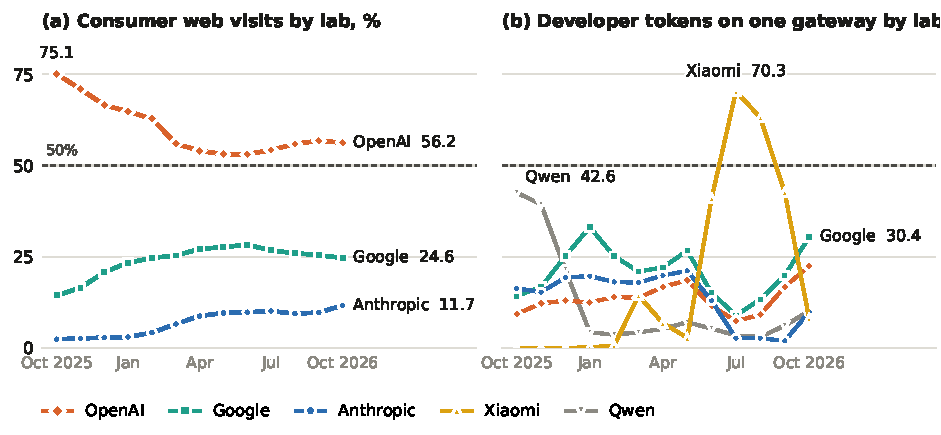
\includegraphics[width=\textwidth]{figs/fig_panel.pdf}
\caption{Thirteen-month panel, October 2025 to October 2026 \cite{aimultiple2026share}. (a) Share of web visits by lab (Similarweb estimates). (b) Share of paid tokens on one gateway by lab, excluding requests made with the customer's own key; only labs that led in some month, and the two largest US labs besides, are drawn. Dashed line: 50\%.}
\label{fig:panel}
\end{figure}

\paragraph{Other series.} The remaining series show the same turnover (Figure~\ref{fig:persist}), a pattern documented independently for the API market \cite{demirer2026emerging}. OpenAI's share of web visits fell from 70.91\% (November 2025) to 54.23\% (July 2026) before recovering to 56.23\% (October) \cite{aimultiple2026share}; the World Bank had measured ChatGPT at 77\% of traffic to the top 60 tools in April 2025 \cite{liu2025who}; ChatGPT's share of combined app and web audience fell below 50\% for the first time in March 2026 \cite{sensortower2026state}. In enterprise API spend OpenAI went from 50\% (2023) to 27\% (2025) and 31\% (2026), while Anthropic went from 12\% to 40\% and 55\% \cite{menlo2026state}; Anthropic passed OpenAI in US business adoption in April 2026 and stood at 44.8\% of businesses against 40.6\% in October \cite{ramp2026index}. On OpenRouter, open weights moved from about 20\% of tokens in 2025 \cite{nagle2025latent} to a peak of 79\% in July 2026, and Qwen's share of paid developer tokens fell from 42.55\% (October 2025) to 3.03\% (August 2026) \cite{aimultiple2026share}. The open-weight share of enterprise usage shows no trend at all: 19\% in early 2025, 13\% by mid-2025 \cite{menlo2025mid}, 11\% later that year and 19\% in 2026 \cite{menlo2026state}. Of the local dominances in Table~\ref{tab:conc}, OpenAI's lost 14.7 points of web-visit share in eleven months and Anthropic's did not exist a year earlier.

\begin{figure}[t]
\centering
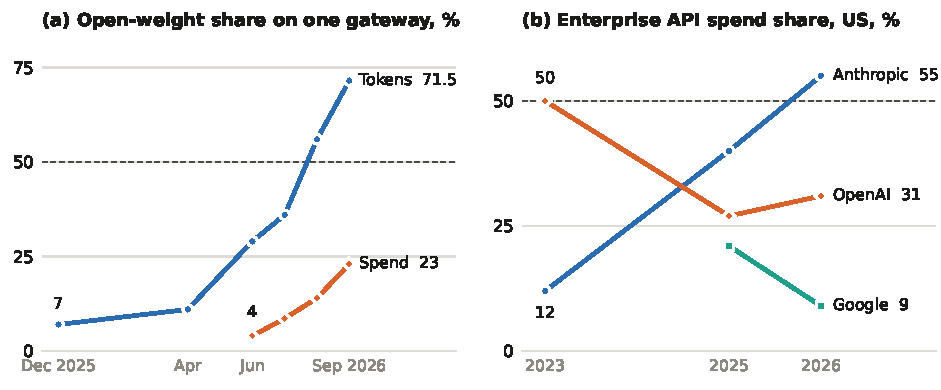
\includegraphics[width=\textwidth]{figs/fig_persist.pdf}
\caption{Two series of leadership change. (a) Open-weight share of tokens and of spend on Vercel's AI Gateway, December 2025 to September 2026 \cite{vercel2026index}. (b) Share of US enterprise LLM API spend, 2023, 2025 and 2026 \cite{menlo2026state}; the source reports no 2023 figure for Google.}
\label{fig:persist}
\end{figure}

\subsection{Upstream layers}
\label{sec:upstream}

The tests in this paper concern adoption. The layers that supply it are more concentrated, and they are outside our data. Analyst estimates place NVIDIA at between 75\% and 86\% of AI accelerator revenue in 2026; no audited market-share figure exists \cite{siliconanalysts2026chain,mordor2026gpu}. On any of those estimates local dominance is not rejected for accelerators at the 50\% threshold. In cloud infrastructure Amazon held 26\%, Microsoft 19\% and Google 16\% of a market of 168 billion dollars in the third quarter of 2026 \cite{synergy2026q3}. No provider reaches 30\%, the three together hold 61\% and the HHI lies between 1{,}293 and 1{,}854. The title of this paper should be read with its subtitle. The claim is that no entity dominates LLM adoption across its dimensions. It is not a claim about the supply of AI, where the accelerator layer has a dominant firm at every threshold used here and where the concentration arguments of the literature are strongest \cite{korinek2025concentrating}.

\section{What the literature changes in the reading of the results}
\label{sec:lit}

The peer-reviewed literature does not reverse any test above. It does change how much weight each result can carry, in six ways.

\paragraph{1. The universal null is stricter than competition law requires.} Law and economics assess dominance within a relevant market \cite{ec2009guidance,kaplow2010why}. If consumer assistants, enterprise APIs and developer inference are distinct relevant markets, as their different prices, buyers and leaders suggest, then no entity should be expected to dominate all of them, and rejecting $\Hzero$ is close to a foregone conclusion. The findings with legal and economic content are the local ones in Table~\ref{tab:conc}. We therefore do not present the universal rejection as evidence of a competitive market. Section~\ref{sec:markets} tests each candidate market separately with second sources: of the three local dominances, one is confirmed at world level, one is confirmed without a stable identity of the leader, and one is not confirmed by a second panel.

\paragraph{2. Concentration with turnover is a known market form.} High concentration without durable dominance is what contestability \cite{baumol1982contestable}, efficiency-based concentration \cite{demsetz1973industry} and competition for the market \cite{schumpeter1942capitalism} describe, and it is what Section~\ref{sec:persist} and the API-market evidence \cite{demirer2026emerging} show. The supply-side literature nevertheless predicts tipping through scale economies and control of complementary assets \cite{korinek2025concentrating,azoulay2025old}, and lock-in theory explains how an early lead can become permanent \cite{katz1985network,arthur1989competing}. A cross-section cannot tell a contestable equilibrium from the early phase of tipping; the OECD reaches the same mixed assessment \cite{oecd2026markets}.

\paragraph{3. Multi-homing weakens the consumer result and not the enterprise one.} As Section~\ref{sec:multihoming} shows, consumers use about 1.5 tools each while firms mostly rely on one model. Of the two local dominances in Western markets, the enterprise one (Anthropic, E) is the one more likely to reflect dependence.

\paragraph{4. Open is not the same as dispersed.} The paradigm test treats open weights as a single entity opposed to closed weights. The literature on openness \cite{widder2024open,azoulay2025old,osborne2024ai} and our own figures (one lab with 62.5\% of top-ten open tokens; Google and Microsoft families leading in enterprises) indicate that the open side is itself concentrated and partly controlled by the same large firms. Section~\ref{sec:openseg} makes the statement more precise. The open side is concentrated by model family (HHI of about 2{,}700 to 3{,}000 on the Hub and 3{,}225 on the gateway) and, because released weights can be served by anyone, unconcentrated by seller (HHI of about 560). Openness spreads the sale of inference, as its defenders expect \cite{kapoor2024societal}, and does not spread the building of models, as its critics expect \cite{widder2024open}; both sides of that debate describe a different count of the same tokens.

\paragraph{5. The token--spend divergence is arithmetic.} A sevenfold to eightfold price gap, together with a price elasticity near one \cite{demirer2025emerging}, reproduces both the 72\% token share and the 23--27\% spend share of open weights. The two metrics are one fact, and neither side's lead in its own metric signals dominance of the market.

\paragraph{6. Unequal intensity is the most robust regularity.} Technology-diffusion research finds that new technologies now arrive everywhere quickly while intensity of use diverges \cite{comin2010exploration,comin2018technology}. Generative AI reached almost all economies within 16 months \cite{liu2024who}, yet the North--South gap widened from 12.1 to 12.6 points in one quarter of 2026 \cite{microsoft2026q2}, and within countries adoption differs by gender \cite{humlum2025unequal,otis2024global}, age \cite{eurostat2025genai}, income and education \cite{cetic2025tic} and firm size \cite{mcelheran2024ai}. This finding holds under every data source used here and does not depend on any vendor's share.

\section{A rival account: three regimes}
\label{sec:rival}

A natural alternative reading of the same sources is that the market consists of three regimes: a Western consumer regime of closed-weight assistants, a Chinese and Global-South regime carried by open-weight Chinese models, and a hybrid enterprise regime. The account is attractive because it assigns each segment a paradigm and an origin. We state it as six propositions and admit each only if (i) its figures can be traced to a primary source and (ii) its prediction survives in the data of Section 5. Table~\ref{tab:rival} gives the outcome.

\begin{table}[t]
\centering\footnotesize
\caption{Counterfactual test of the three-regime account. Each row states a proposition the account implies, the evidence assembled here that bears on it, and the outcome. Of the six propositions two hold, two fail and two survive only in a narrower form, which is why the account is reported as a partial rival rather than an alternative explanation.}
\label{tab:rival}
\begin{tabularx}{\textwidth}{@{}l L{4.3cm} X l@{}}
\toprule
& Proposition & Test and evidence & Outcome \\
\midrule
P1 & Market share depends on the layer measured. & Open-weight or China-origin share by layer, two vintages. 2025: 30\% of gateway tokens, 13\% of enterprise usage, about 7\% of web visits. 2026: 72\%, 19\%, 4.2\%. The ordering is the same in both years. & Holds \\
P2 & The Chinese consumer market is an open-weight regime. & The leading app, Doubao, holds 54.3\% of top-five MAU and belongs to ByteDance, which is absent from the open-weight labs in every gateway ranking used here. Apps of open-weight labs (Qwen, DeepSeek) hold 36.4\%. & Fails \\
P3 & Open-weight Chinese models carry adoption in the Global South. & DeepSeek's share is 1.0--2.6\% in the seven Global-South markets measured (median 1.6\%), against a median of 1.0\% in ten Northern markets. It leads only where US services are restricted: China, Belarus, Cuba, Russia (Figure~\ref{fig:access}). & Narrower form \\
P4 & Without programming workloads the open-weight share would fall. & No source reports shares net of programming. The 2025 study the claim rests on reports the opposite composition: role-play was about 52\% of open-source tokens \cite{aubakirova2026state}. & Fails \\
P5 & Restrictive licences on Western open models explain their low enterprise use. & Licences do differ and ``open'' is not one category \cite{schrepel2025measuring,duan2025position}. The causal claim is contradicted: Gemma, Phi and Llama lead enterprise production use, ahead of DeepSeek and Qwen \cite{futurum2026open}. & Narrower form \\
P6 & Enterprises use open weights widely and pay little for them. & 63\% of organisations use an open model \cite{mckinsey2025open}; 42\% run one in production \cite{futurum2026open}; 19\% of usage and 4\% of spend \cite{menlo2026state}. & Holds \\
\bottomrule
\end{tabularx}
\end{table}

\begin{figure}[t]
\centering
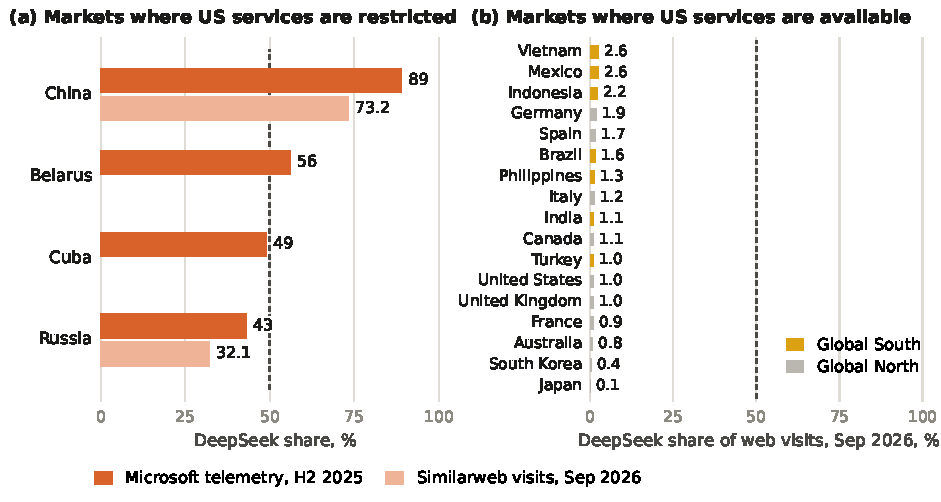
\includegraphics[width=\textwidth]{figs/fig_access.pdf}
\caption{DeepSeek's share by market access. (a) Economies in which Microsoft reports the highest DeepSeek shares, all of them markets where US services face restrictions \cite{microsoft2026h2}; lighter bars give the Similarweb share among seven assistants where available. (b) The 17 other economies in Appendix~\ref{app:geo}. The two sources use different definitions of share.}
\label{fig:access}
\end{figure}

Two propositions hold, two hold only in a narrower form and two fail. The account is right that share is layer-dependent (P1), which is the thesis of this paper and replicates across two annual vintages, and right about enterprises (P6). It is wrong to equate the Chinese market with open weights (P2) and has no support for its programming counterfactual (P4).

\paragraph{The access counterfactual.} The informative case is P3. Microsoft reports DeepSeek shares of 89\% in China, 56\% in Belarus, 49\% in Cuba and 43\% in Russia, says that demand is strongest where US services face restrictions, and describes adoption in North America and Europe as low \cite{microsoft2026h2}. Similarweb gives 73.2\% for China and 32.1\% for Russia among seven assistants. In the 17 economies where US assistants are available, DeepSeek's share is between 0.1\% and 2.6\%, with a median of 1.1\%, and US-origin assistants hold between 97.4\% and 99.0\% of visits in India, Brazil, Indonesia, Vietnam, Mexico, the Philippines and Turkey. The dividing line is therefore access and not income: where both origins are available, China-origin models are a marginal consumer choice in the Global South as in the North. This sharpens the origin-level result of Section~\ref{sec:origin}. The same report notes that African usage of DeepSeek is two to four times that of other regions; that is a relative statement and does not establish leadership there.

\paragraph{Figures not used.} In assembling this account we could not trace the following figures to a primary source and do not use them: DeepSeek shares for Iran, Syria and individual African countries (the Microsoft report names Iran as a strong market without a figure); and an open-weight share of 30\% of adoption in the Global South.

\section{Threats to validity}
\label{sec:validity}

\paragraph{Construct validity.} A ``user'' is an account, a device or a survey respondent depending on the source. Counterpoint's vendor MAUs sum to about 4.8 billion \cite{counterpoint2026mau}. Microsoft's 18.8\% of a working-age population of about 5.3 billion \cite{un2024wpp} is about 1.0 billion people, fewer than ChatGPT's claimed weekly users alone. The two cannot both describe unique humans. Embedded assistants change the ranking: Counterpoint counts Meta AI and places Meta first, whereas DataReportal excludes use inside WhatsApp, Office or Snapchat \cite{datareportal2026}. ``Open'' and ``closed'' are properties of models, and several labs ship both; classification by lab is an approximation, and we did not verify the licence of the model currently behind Meta AI, which alone would move more than a billion estimated users between columns.

\paragraph{Measurement validity.} Independent sources disagree by large factors on nominally identical constructs: China's adoption is 17.5\% according to Microsoft and above 50\% according to the CNNIC (ratio 2.9); US weekly use is 33.0\% by telemetry and 49\% by survey (ratio 1.5); Google's developer share is 15.1\% of requests and 30.4\% of paid tokens. Microsoft itself expects its next edition to raise the figure for China more than for other economies \cite{microsoft2026q2}. Trackers of the same construct disagree as well (Table~\ref{tab:trackers}): StatCounter, whose figures are based on referral tracking, gives ChatGPT 79.4\% and DeepSeek 0.02\% of the consumer chat market \cite{statcounter2026}, where Similarweb's visit counts give 56.6\% and 3.5\%. The leader and its local dominance in A survive the change of tracker (in Brazil StatCounter gives ChatGPT 80.5\% against Similarweb's 65.1\%); every other share moves by a factor of two or more, DeepSeek's by a factor of 175, and the HHI of metric A rises from 3{,}968 to about 6{,}460.

\begin{table}[h]
\centering\small
\caption{Two trackers of consumer chat share (\%). Similarweb: web visits among seven assistants, October 2026 \cite{momentic2026chatbots}. StatCounter: referral-based share, August 2026 \cite{statcounter2026}.}
\label{tab:trackers}
\begin{tabular}{@{}lrrr@{}}
\toprule
Assistant & Similarweb & StatCounter & Ratio of larger to smaller \\
\midrule
ChatGPT & 56.6 & 79.4 & 1.4 \\
Gemini & 24.7 & 10.9 & 2.3 \\
Claude & 11.7 & 2.57 & 4.6 \\
DeepSeek & 3.5 & 0.02 & 175 \\
Perplexity & 0.8 & 4.31 & 5.4 \\
Copilot & 0.7 & 2.79 & 4.0 \\
\bottomrule
\end{tabular}
\end{table}

 The tolerance $\kappa^{*}=2$ was chosen with these ratios in view, and results that depend on a smaller margin are reported as inconclusive.

\paragraph{Coverage.} Gateways observe a small fraction of global inference (Section~\ref{sec:paradigm}) and miss first-party APIs, enterprise contracts, on-premises and on-device use. Web panels miss apps and embedded AI. The layer in which small open models are actually run, on premises and on devices, is observed only through downloads, which count requests and include automated pulls \cite{lambert2026atom}. For Africa we found a single regional aggregate, from a tracker of page views (Section~\ref{sec:markets}), and no survey or telemetry by country. No source reports tokens by country of user. Enterprise spend is measured for the United States and, through one card platform, for Europe; first-party API volumes, self-hosted inference and assistants embedded in other products remain outside every share metric used here.

\paragraph{Source interest.} Menlo Ventures invests in Anthropic and in OpenRouter \cite{menlo2026state}; OpenRouter, Vercel and Ramp publish data from their own platforms; OpenAI, Google and ByteDance report their own user and token counts; the CNNIC is a state body. Andreessen Horowitz invests in OpenAI \cite{a16z2026cio}, and its survey and Menlo's name different leaders for the same market; Moss reports the spending of its own customers; AICPB does not document its panel. We mitigate this by requiring two sources of different type per claim, and note where only one exists (dimension E outside the US; all of G). Two sources used in Section~\ref{sec:openseg} have a direct stake. The 30-day Hub download shares are published by the maintainer of the leaderboard that produces them \cite{vidraft2026top300}; we rely on them only where the ATOM report and Hugging Face's own figures point the same way. The provider shares come from a firm that finances GPUs for inference hosts \cite{amcompute2026providers}; they have no independent replication, and the coding of headquarters is the source's.

\paragraph{Temporal validity.} Metrics span April to November 2026. Given the turnover documented in Section~\ref{sec:persist}, a cross-section mixing months can mislabel leaders in fragile dimensions (B and C). The robust-lead analysis addresses this in part, and the thirteen-month panel covers only two of the four candidate markets. One tracker changed its worldwide figure for the leading assistant by 28 points in two months (Section~\ref{sec:markets}), which no other source corroborates.

\paragraph{Statistical validity.} The tolerance rule has a false-rejection rate of 11\% at the reference error scale (Section~\ref{sec:vendor}), so its verdicts are not tests at the 5\% level. The pooled test controls its error rate only under the assumed model: log-normal errors of known and common scale, independent across dimensions or sharing a vendor-level component. The scale is not estimated from data, and a common bias affecting all vendors in one dimension is not modelled. A single share carries little information at that scale, since a local null is rejected only when the leader is below 28.1\%; verdicts on single metrics are weak in both directions, and the conclusions that carry weight are those that pool dimensions. At the paradigm and origin levels the metrics pooled are not independent (two gateways, three enterprise sources), which is why we also report the grouped version. The partial-ownership adjustment assumes the Cournot setting of \cite{obrien2000competitive}, and the stake attributed to Microsoft was read from summaries of its filing. Metrics within a dimension are correlated (E and E$'$; D and D$'$ share a platform), so the eight-metric $W$ overstates the evidence. The split of ``others'' and the imputation of unlisted shares (Meta in D, open-source labs in E) affect ranks at the bottom of the table only. In Section~\ref{sec:openseg}, concentration by seller is reconstructed from two tables that the source does not reconcile: its family table sums to 145.9 trillion tokens and implies a total of 151.6 trillion, while our seller total is 144.6 trillion. The reconstruction covers one router in one week, and the HHI of about 560 should be read as an order of magnitude. The rank tests on families use six entities and have almost no power; enterprise use is a multiple-response percentage and enters those tests as a rank only.

\paragraph{External validity.} The result describes adoption shares in 2026. It says nothing about control of compute, chips or data, where concentration arguments are strongest \cite{korinek2025concentrating}.

\section{Discussion and conclusion}

On single-source data universal dominance at 50\% is rejected at the vendor level under every specification with independent measurement errors, and under correlated errors in the primary specification only. At 40\% it is rejected only with independent errors, and at 30\% it is not rejected. The rejection does not survive the most adverse reading of the evidence: with the most favourable source in each dimension the calibrated test gives $p$ between 0.07 and 0.16, and if, on that reading, Google and Anthropic are counted as one entity, a 30\% threshold is met in every dimension. At the paradigm and origin levels the test separates the two sides: dominance by open weights and by China-origin labs is rejected, and dominance by closed weights and by US-origin labs is not, because their shares fall below 50\% only in gateway tokens and open-model downloads and by less than the error tolerance. The data do not support the looser statement that the LLM market is unconcentrated, and Section~\ref{sec:lit} argues that the universal rejection is the least informative of the results. The picture that fits all nine metrics is a set of segments, each with a different leader and each highly concentrated: OpenAI in consumer attention, Meta, OpenAI and Google close together in reach, Anthropic in enterprise spend on four of five sources and narrowly in revenue, DeepSeek, Google or OpenAI in developer volume according to the unit, ByteDance in China on one of two panels. The pattern repeats one level down, inside the open-weight segment: Qwen on the Hub and in local inference, DeepSeek on the gateway, Gemma in enterprise production (Section~\ref{sec:openseg}). Which of these one calls ``the market'' determines who appears dominant. Origin adds one conditional: China-origin models lead consumer use where US services are restricted and are marginal wherever both are available, in the Global South as in the North (Section~\ref{sec:rival}).

Three implications follow. For measurement, any claim of dominance should name its unit, its market and its source, and token share in particular should not be read as market share: it moved by tens of points within a quarter under price promotions, and it differs from spend share by exactly the price gap. For open weights there is a further gap between the share of a model family and the share of a firm: about two thirds of open-weight gateway tokens are sold by firms other than the lab that released the weights, and more than half of the tokens of Chinese families are sold by hosts headquartered in the United States. For policy, the relevant antitrust question is segment-specific: the evidence is strongest for consumer chat outside China, where one assistant leads 17 of 19 countries (although its users multi-home), and for enterprise APIs, where firms single-home; it is weakest for developer inference. For diffusion, the sharper divide is between populations (Section~\ref{sec:geo}): adoption in the Global North is 12.6 points above the Global South, and inside Brazil the gap between the top and bottom income classes is 53 points. On that axis no vendor's share matters as much as who is using any model at all. None of this extends upstream: in AI accelerators one firm holds a share that meets every threshold used here (Section~\ref{sec:upstream}).

The next step is a preregistered replication on a fixed monthly panel, with the assumed error model replaced by estimated uncertainty, which requires what no publisher currently provides: deduplicated users, tokens by country of user, and volumes for self-hosted inference.

\section*{Data and code availability}
All inputs are published figures cited in the text. Everything needed to reproduce the article is in the public replication package \cite{oliveira2026repo} at \url{https://github.com/rfapo/no-universal-ai-dominance}, and the file names used throughout this article are paths in that repository. \texttt{code/analysis.py} carries every transcribed input and produces every statistic reported here (HHI bounds, robustness margins, Kendall's $W$ with its permutation test, the measurement-error simulation, the calibrated pooled test, the bloc scenarios, the panel statistics and the implied price ratios), writing them to \texttt{results/results.json}. \texttt{code/validate\_stats.py} re-implements each statistical procedure by a different route---Kendall's $W$ through the Friedman statistic, the pooled test with a different seed and a larger simulation, the partial-ownership HHI through the general formula of O'Brien and Salop rather than its closed form, the HHI upper bound against a brute-force search over admissible splits of the unattributed residual---and records the comparison in \texttt{results/validation.json}; it also reports the size and power of the pooled test at the least favourable point of the null. \texttt{code/figures.py} draws the fourteen figures, \texttt{data/sources.csv} lists the URL behind every data source, and \texttt{code/archive\_urls.sh} requests an Internet Archive snapshot of each. The \LaTeX{} source of this article is in \texttt{paper/}. The repository adds a test suite (\texttt{tests/test\_paper\_claims.py}) that checks every number quoted in the tables and in the prose against \texttt{results/results.json}, so that a drift between the script and the manuscript fails, and a continuous-integration workflow that re-runs the analysis from scratch on each change. Every simulation is seeded, so \texttt{results/results.json} and \texttt{results/validation.json} reproduce byte for byte on any platform, which the workflow confirms on Linux against outputs produced on macOS; the rendered figures depend in addition on the versions of Matplotlib, Pillow and FreeType and on the fonts the host has installed, so the check requires that they be redrawn at the reference dimensions and reports any difference in pixels.

\section*{AI assistance and competing interests}
Source discovery and literature searches were run by the author on four AI assistants from different vendors and countries of origin (DeepSeek, Qwen, Gemini and Claude), so that the selection of sources would not depend on a single model. The analysis scripts and the draft of the manuscript were produced with Claude (Anthropic). The four vendors are among those analysed here, and a Claude model ranks first on two of the leaderboards cited; readers should weigh this. The author is responsible for the content and for checking every figure against its source. This research received no funding.

\clearpage
\appendix
\section{Coverage audit: ten gap and counterfactual questions}
\label{app:audit}

\begin{table}[H]
\centering\footnotesize
\caption{Questions used to audit source coverage before the analysis, and their outcome.}
\begin{tabularx}{\textwidth}{@{}r L{6.1cm} X@{}}
\toprule
& Question & Outcome \\
\midrule
1 & What fraction of global tokens passes through the gateways behind the ``open weights won'' claim? & Covered. About 6\% of the sum of two first-party providers alone (Section~\ref{sec:paradigm}). \\
2 & Who leads if the weight is dollars and not tokens? & Covered. Closed weights in every source. \\
3 & Do Western panels observe China? & Partial. They do not; CNNIC and QuestMobile were added but cannot be audited. \\
4 & Does embedded AI (Meta AI, AI Overviews, Copilot) count as use? & Partial. It changes the ranking and sources differ. \\
5 & Are summed MAUs unique people? & Open. No source deduplicates globally. \\
6 & What about self-hosted, on-premises and on-device use? & Partial. Downloads and surveys exist; token volumes do not. \\
7 & Does the publisher have a stake in the result? & Covered. Flagged in Tables~\ref{tab:data} and~\ref{tab:markets} and in Section~\ref{sec:validity}; two investor-run surveys name different leaders. \\
8 & Is token share stable under promotions and free tiers? & Covered. It is not (Section~\ref{sec:persist}). \\
9 & Can ``open'' and ``closed'' be assigned by lab? & Partial. Several labs ship both. \\
10 & Is there primary data for the Global South, Brazil, Africa and non-English users? & Partial. Brazil yes; for Africa one regional aggregate from a page-view tracker (Section~\ref{sec:markets}). \\
\bottomrule
\end{tabularx}
\end{table}

\section{Concentration measured at other weightings of the leader}
\label{app:hill}

The HHI is one member of a family. The Hill number of order $q$,
\[
{}^{q}N=\Big(\textstyle\sum_i p_i^{\,q}\Big)^{1/(1-q)},\qquad
{}^{1}N=\exp\!\Big(-\textstyle\sum_i p_i\ln p_i\Big),
\]
counts the equally sized firms that would reproduce the observed concentration, and $q$ sets how heavily the largest firms are weighted. The family spans the indices in common use: ${}^{0}N$ is the number of firms, ${}^{1}N$ is the exponential of the Shannon entropy, ${}^{2}N$ is $1/\mathrm{HHI}$ and ${}^{\infty}N$ is $1/s_{(1)}$. Reporting the profile rather than a single index shows how far a verdict depends on a choice that is rarely argued for.

Table~\ref{tab:hill} gives the profile for the nine metrics. Shares are renormalised over the named firms, so the unattributed residual is treated as if it did not exist; this is the concentration-maximising convention, and it is why ${}^{2}N$ here is below the $1/\mathrm{HHI}$ column of Table~\ref{tab:conc}, which credits the residual with competitors. The last column gives the residual, and the gap between the two readings grows with it.

\begin{table}[h]
\centering\small
\caption{Effective number of competitors at four weightings of the leader. ${}^{2}N=1/\mathrm{HHI}$. Residual: share not attributed to a named firm (\%).}
\label{tab:hill}
\begin{tabular}{@{}lrrrrr@{}}
\toprule
& ${}^{0}N$ & ${}^{1}N$ & ${}^{2}N$ & ${}^{\infty}N$ & residual \\
& firms & $\exp(H)$ & $1/\mathrm{HHI}$ & $1/s_{(1)}$ & \\
\midrule
A & 7 & 3.27 & 2.52 & 1.77 & 0.1 \\
B & 7 & 5.52 & 4.80 & 3.53 & 11.7 \\
C & 12 & 5.81 & 4.36 & 3.03 & 4.9 \\
D & 9 & 6.14 & 4.85 & 2.89 & 8.1 \\
E & 3 & 2.47 & 2.22 & 1.73 & 5.0 \\
D$'$ & 10 & 6.41 & 5.03 & 3.08 & 6.4 \\
E$'$ & 4 & 2.37 & 2.17 & 2.02 & 0.5 \\
F & 3 & 2.59 & 2.35 & 1.82 & 15.6 \\
G & 5 & 3.44 & 2.73 & 1.84 & 0.0 \\
\bottomrule
\end{tabular}
\end{table}

Two readings survive the whole profile and one does not. The separation between the concentrated metrics (A, E, E$'$, F, G) and the rest holds at every $q\ge1$ ---the largest of the first group stays below the smallest of the second---so calling consumer attention and enterprise spend concentrated does not depend on the weighting. It does not hold at $q=0$, which counts firms and ignores their sizes, and where A and B both show seven. The \emph{ordering} within that group does not hold: E$'$ is the most concentrated metric at $q=2$ (${}^{2}N=2.17$) and the least concentrated of the five at $q=\infty$ (${}^{\infty}N=2.02$), because its two leaders are nearly equal, while E has the smaller leader-based count (1.73) on a larger index. Rankings by HHI and by leader's share therefore disagree, and a paper that reports only one of them is making a choice it has not declared. Metrics C and D show the complementary pattern: twelve and nine named firms give ${}^{0}N$ far above ${}^{2}N$, the signature of a long tail that the index correctly discounts.

This is the same point the paper makes about units, applied one level down. The unit of measurement changes who leads; the weighting inside the concentration index changes which market looks tightest.

\section{Assistant shares by country}
\label{app:geo}

\begin{table}[H]
\centering\footnotesize
\caption{Share (\%) of web visits among seven assistants, September 2026 (United States: October 2026). Source: Similarweb estimates compiled by \cite{momentic2026chatbots}. HHI computed within the seven.}
\begin{tabular}{@{}lrrrrrrrr@{}}
\toprule
Country & ChatGPT & Gemini & Claude & DeepSeek & Grok & Perplexity & Copilot & HHI \\
\midrule
United States & 62.9 & 16.5 & 14.8 & 1.0 & 2.6 & 1.1 & 1.1 & 4{,}458 \\
India & 64.1 & 20.2 & 11.7 & 1.1 & 1.7 & 0.9 & 0.2 & 4{,}659 \\
Japan & 55.6 & 35.5 & 6.3 & 0.1 & 1.1 & 0.4 & 1.0 & 4{,}394 \\
Brazil & 65.1 & 26.3 & 4.7 & 1.6 & 1.5 & 0.4 & 0.5 & 4{,}957 \\
Indonesia & 49.4 & 34.8 & 11.0 & 2.2 & 1.7 & 0.8 & 0.2 & 3{,}781 \\
United Kingdom & 68.2 & 14.3 & 13.0 & 1.0 & 1.5 & 0.9 & 1.1 & 5{,}030 \\
South Korea & 56.5 & 30.6 & 9.8 & 0.4 & 2.0 & 0.5 & 0.2 & 4{,}229 \\
Germany & 62.6 & 21.5 & 9.8 & 1.9 & 1.9 & 1.6 & 0.7 & 4{,}487 \\
France & 62.5 & 21.4 & 12.0 & 0.9 & 1.1 & 1.3 & 0.7 & 4{,}512 \\
Canada & 64.3 & 19.3 & 11.6 & 1.1 & 1.8 & 1.1 & 0.8 & 4{,}648 \\
Vietnam & 46.8 & 43.5 & 3.4 & 2.6 & 3.3 & 0.1 & 0.2 & 4{,}112 \\
Mexico & 47.1 & 39.2 & 7.3 & 2.6 & 2.5 & 0.6 & 0.7 & 3{,}822 \\
China & 17.7 & 5.5 & 1.3 & 73.2 & 1.8 & 0.5 & 0.1 & 5{,}707 \\
Philippines & 62.2 & 25.7 & 8.4 & 1.3 & 0.9 & 0.8 & 0.7 & 4{,}604 \\
Spain & 55.0 & 29.7 & 10.0 & 1.7 & 1.5 & 1.1 & 1.0 & 4{,}014 \\
Italy & 43.5 & 44.8 & 7.8 & 1.2 & 0.8 & 0.9 & 1.0 & 3{,}964 \\
Australia & 66.6 & 12.5 & 15.5 & 0.8 & 1.9 & 1.0 & 1.7 & 4{,}840 \\
Turkey & 48.4 & 43.0 & 5.8 & 1.0 & 1.3 & 0.2 & 0.2 & 4{,}228 \\
Russia & 43.6 & 13.7 & 4.5 & 32.1 & 2.3 & 3.6 & 0.2 & 3{,}158 \\
\bottomrule
\end{tabular}
\end{table}

\bibliographystyle{unsrtnat}
\bibliography{references}

\end{document}
